%% This is the ctufit-thesis example file. It is used to produce theses
%% for submission to Czech Technical University, Faculty of Information Technology.
%%
%% This is version 1.3.10, built 27. 2. 2025.
%% 
%% Get the newest version from
%% https://gitlab.fit.cvut.cz/theses-templates/FITthesis-LaTeX
%%
%%
%% Copyright 2024, Tomas Novacek
%% Copyright 2021, Eliska Sestakova and Ondrej Guth
%%
%% This work may be distributed and/or modified under the
%% conditions of the LaTeX Project Public License, either version 1.3
%% of this license or (at your option) any later version.
%% The latest version of this license is in
%%  https://www.latex-project.org/lppl.txt
%% and version 1.3 or later is part of all distributions of LaTeX
%% version 2005/12/01 or later.
%%
%% This work has the LPPL maintenance status `maintained'.
%%
%% The current maintainer of this work is Tomas Novacek.
%% Alternatively, submit bug reports to the tracker at
%% https://gitlab.fit.cvut.cz/theses-templates/FITthesis-LaTeX/issues
%%
%%

% arara: xelatex
% arara: biber
% arara: xelatex
% arara: xelatex

%%%%%%%%%%%%%%%%%%%%%%%%%%%%%%%%%%%%%%%%%
% CLASS OPTIONS
% language: czech/english/slovak
% thesis type: bachelor/master/dissertation
% colour: bw for black&white OR no option for default colour scheme
% electronic (oneside) or printed (twoside), twoside is default
% paragraph - if passed, this optional argument sets paragraphs as the deepest level of headers, styles it, numbers it and adds it to Table of Content. Use with care! Normally, it is considered unwise to use it, since its too deep.
%%%%%%%%%%%%%%%%%%%%%%%%%%%%%%%%%%%%%%%%%
\documentclass[czech,master,unicode,oneside]{ctufit-thesis}

%%%%%%%%%%%%%%%%%%%%%%%%%%%%%%%%%%
% FILL IN THIS INFORMATION
%%%%%%%%%%%%%%%%%%%%%%%%%%%%%%%%%%
\ctufittitle{Porovnání Frama-C a Stainless} % replace with the title of your thesis
\ctufitauthorfull{Bc. Luboš Zápotočný} % replace with your full name (first name(s) and then family name(s) / surname(s)) including academic degrees
\ctufitauthorsurnames{Zápotočný} % replace with your surname(s) / family name(s)
\ctufitauthorgivennames{Luboš} % replace with your first name(s) / given name(s)
\ctufitsupervisor{doc.\,RNDr.\,Dušan Knop,\,Ph.D.} % replace with name of your supervisor/advisor (include academic degrees)
\ctufitdepartment{Katedra teoretické informatiky} % replace with the department of your defence
\ctufityear{2025} % replace with the year of your defence
\ctufitdeclarationplace{Praze} % replace with the place where you sign the declaration
\ctufitdeclarationdate{\today} % replace with the date of signature of the declaration
% TODO: vylepsit
\ctufitabstractCZE{
Formální verifikace se zabývá dokazováním správnosti programů na základě matematických metod a logiky. Ověřené programy díky tomu poskytují záruku, že pracují v souladu s předem definovanou specifikací za všech okolností, a výrazně tak snižují riziko kritických chyb, které by tradiční testování mohlo přehlédnout.

Tato diplomová práce se věnuje teoretickým aspektům formální verifikace a studiu dostupných nástrojů pro automatizované dokazování (SMT řešičů), jako jsou Alt-Ergo, CVC4/5 a Z3, a jejich integraci v prostředích Frama-C (pro jazyk C) a Stainless (pro jazyk Scala). Zároveň porovnává přístupy obou nástrojů na praktickém příkladu formálně verifikované implementace datové struktury AVL stromu, přičemž zvláštní důraz klade na rozbor rozdílů v dokazování pomocí těchto dvou frameworků.
}
\ctufitabstractENG{
Formal verification focuses on proving program correctness using mathematical methods and logic. Verified programs therefore guarantee that they behave according to a predefined specification under all circumstances, markedly reducing the risk of critical errors that traditional testing could overlook.

This thesis explores the theoretical aspects of formal verification and investigates the available automated-proving tools (SMT solvers) such as Alt-Ergo, CVC4/5, and Z3, along with their integration within the Frama-C environment (for the C language) and Stainless (for Scala). It also compares the approaches of these two toolchains through a practical case study: a formally verified implementation of the AVL-tree data structure, with special emphasis on analysing the differences in proof development across the two frameworks.
}
\ctufitkeywordsCZE{formalní verifikace, SMT, Frama-C, Stainless}
\ctufitkeywordsENG{formal verification, SMT, Frama-C, Stainless}
%%%%%%%%%%%%%%%%%%%%%%%%%%%%%%%%%%
% END FILL IN
%%%%%%%%%%%%%%%%%%%%%%%%%%%%%%%%%%

%%%%%%%%%%%%%%%%%%%%%%%%%%%%%%%%%%
% CUSTOMIZATION of this template
% Skip this part or alter it if you know what you are doing.
%%%%%%%%%%%%%%%%%%%%%%%%%%%%%%%%%%

\RequirePackage{iftex}[2020/03/06]
\iftutex % XeLaTeX and LuaLaTeX
    \RequirePackage{ellipsis}[2020/05/22] %ellipsis workaround for XeLaTeX
\else
    \errmessage{Only compilation with XeLaTeX or LuaLaTeX is allowed}
    \stop
\fi

% hyperlinks
\hypersetup{
    pdfpagelayout=TwoPageRight,
    colorlinks=false,
    allcolors=decoration,
    pdfborder={0 0 0.1}
}

% uncomment the following to hide all hyperlinks
%\hypersetup{hidelinks}

% uncomment the following to change the colour of all hyperlinks to CTU blue
%\hypersetup{allbordercolors=decoration}

\RequirePackage{pdfpages}[2020/01/28]

%%%%%%%%%%%%%%%%%%%%%%%%%%%%%%%%%%
% CUSTOMIZATION of this template END
%%%%%%%%%%%%%%%%%%%%%%%%%%%%%%%%%%


%%%%%%%%%%%%%%%%%%%%%%
% DEMO CONTENTS SETTINGS
% You may choose to modify this part.
%%%%%%%%%%%%%%%%%%%%%%
\usepackage{dirtree}
\usepackage{lipsum,tikz}
\usepackage[style=iso-numeric]{biblatex}
\addbibresource{text/bib-database.bib}
\usepackage{xurl}
\usepackage{listings} % typesetting of sources
\usepackage{minted}
\usepackage{csquotes}
\usepackage{float} % for [H] placement of figures

%%%%%%%%%%%%%%%%%%%%%%
% DEMO CONTENTS SETTINGS END
%%%%%%%%%%%%%%%%%%%%%%

\begin{document} 
\frontmatter\frontmatterinit % do not remove these two commands

\thispagestyle{empty}\maketitle\thispagestyle{empty}\cleardoublepage % do not remove these four commands

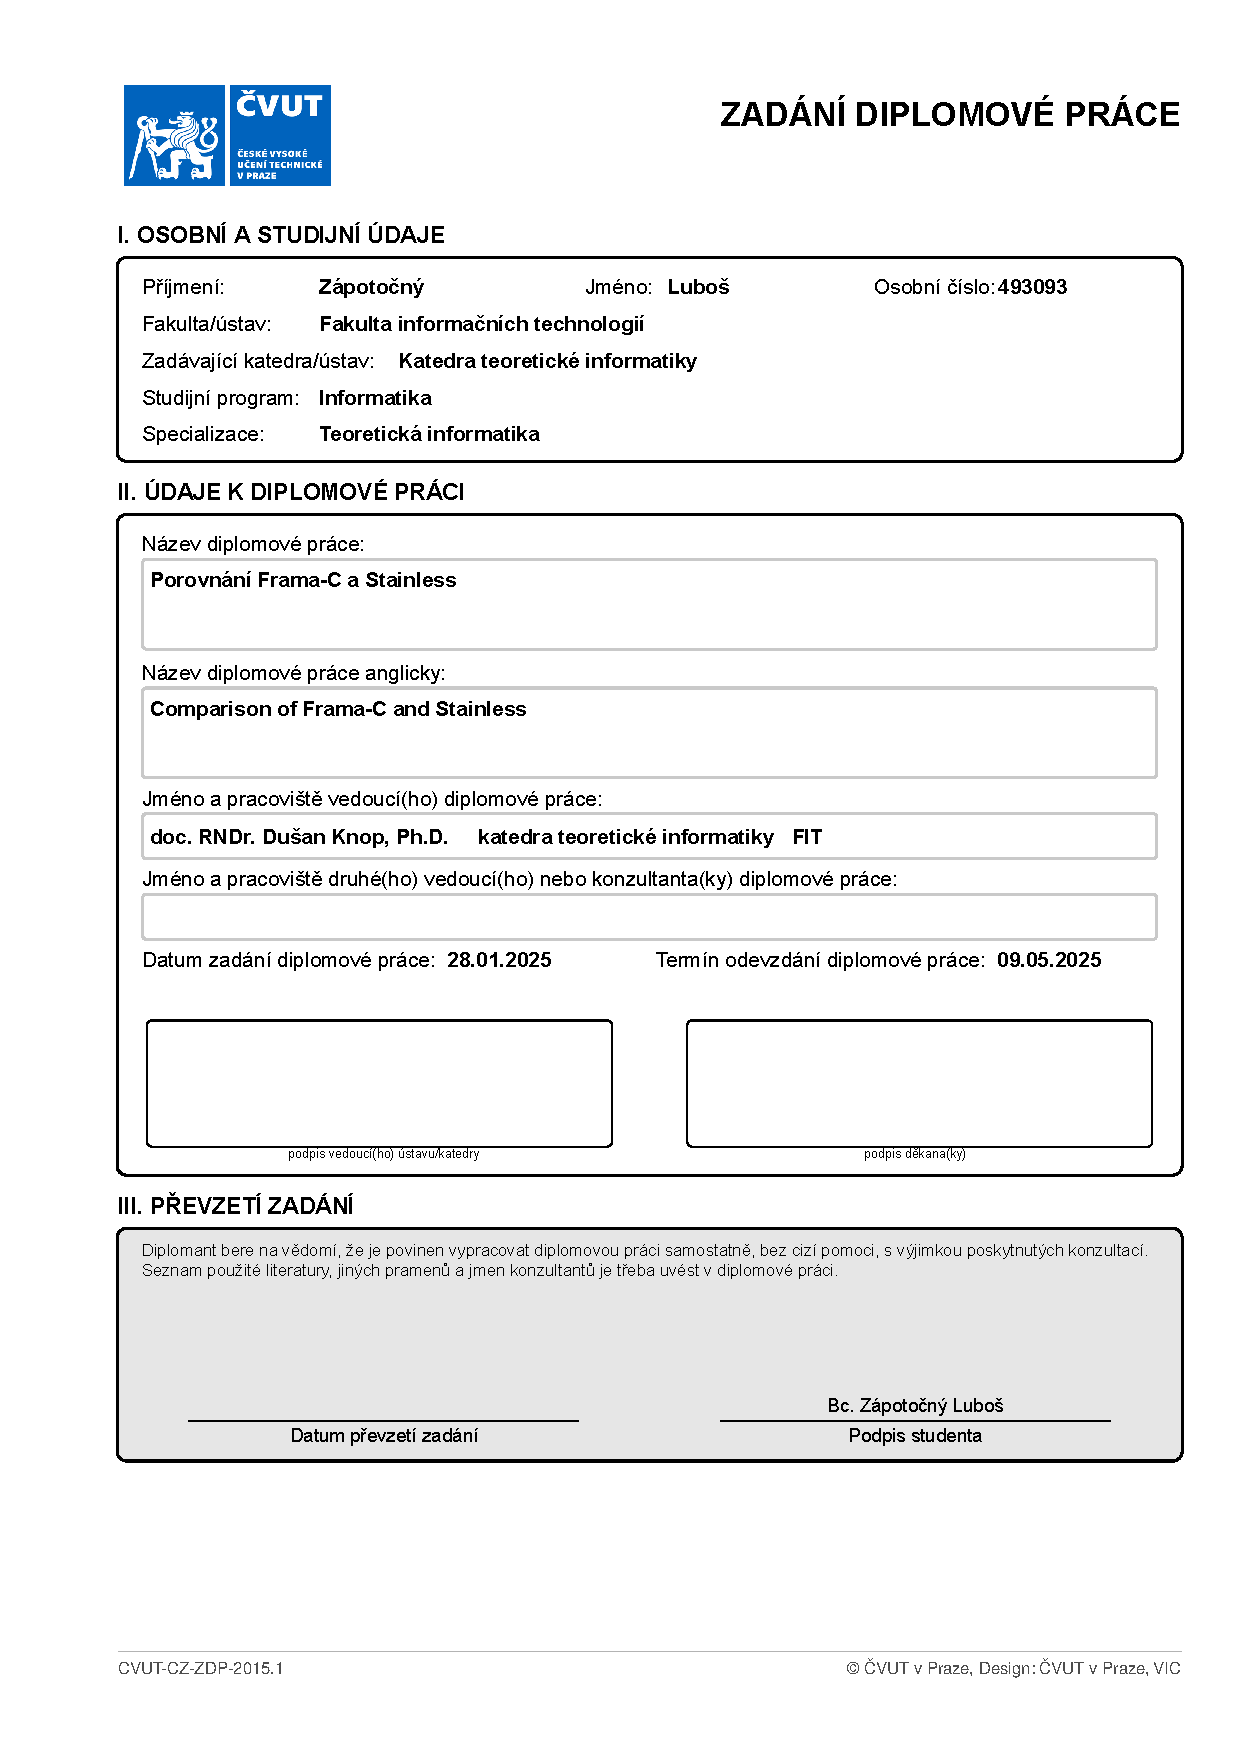
\includepdf[pages={1-}]{zapotlub-assignment.pdf} % replace this file with your thesis assignment generated from ProjectsFIT

\imprintpage % do not remove this command
\stopTOCentries
%%%%%%%%%%%%%%%%%%%%%%
% list of other contents END
%%%%%%%%%%%%%%%%%%%%%%

%%%%%%%%%%%%%%%%%%%
% ACKNOWLEDGMENT
% FILL IN / MODIFY
% This is a place to thank people for helping you. It is common to thank your supervisor.
%%%%%%%%%%%%%%%%%%%
\begin{acknowledgmentpage}
    Chtěl bych poděkovat blízkým za podporu během celého studia.
    Dále bych chtěl bych poděkovat doc. RNDr. Dušanovi Knopovi, Ph.D. za odborné vedení diplomové práce.
\end{acknowledgmentpage}
%%%%%%%%%%%%%%%%%%%
% ACKNOWLEDGMENT END
%%%%%%%%%%%%%%%%%%%


%%%%%%%%%%%%%%%%%%%
% DECLARATION
% FILL IN / MODIFY
%%%%%%%%%%%%%%%%%%%
% INSTRUCTIONS
% ENG: choose one of approved texts of the declaration. DO NOT CREATE YOUR OWN. Find the approved texts at https://courses.fit.cvut.cz/SFE/download/index.html#_documents (document Declaration for FT in English)
% CZE/SLO: Vyberte jedno z fakultou schvalenych prohlaseni. NEVKLADEJTE VLASTNI TEXT. Schvalena prohlaseni najdete zde: https://courses.fit.cvut.cz/SZZ/dokumenty/index.html#_dokumenty (prohlášení do ZP)
\begin{declarationpage}
Prohlašuji, že jsem předloženou práci vypracoval samostatně a že jsem uvedl veškeré použité
informační zdroje v souladu s Metodickým pokynem o dodržování etických principů při přípravě
vysokoškolských závěrečných prací.

Beru na vědomí, že se na moji práci vztahují práva a povinnosti vyplývající ze zákona č. 121/2000 Sb.,
autorského zákona, ve znění pozdějších předpisů, zejména skutečnost, že České vysoké učení
technické v Praze má právo na uzavření licenční smlouvy o užití této práce jako školního díla podle §
60 odst. 1 citovaného zákona.

Prohlašuji, že jsem v průběhu příprav a psaní závěrečné práce použil nástroje umělé
inteligence. Vygenerovaný obsah jsem ověřil. Stvrzuji, že jsem si vědom, že za obsah
závěrečné práce plně zodpovídám.
\end{declarationpage}
%%%%%%%%%%%%%%%%%%%
% DECLARATION END
%%%%%%%%%%%%%%%%%%%

\printabstractpage % do not remove this command

%%%%%%%%%%%%%%%%%%%
% SUMMARY
% FILL IN / MODIFY
% OR REMOVE ENTIRELY (upon agreement with your supervisor)
% (appropriate to remove in most theses)
%%%%%%%%%%%%%%%%%%%
% \begin{summarypage}
% \section*{Summary section}
% 
% \lipsum[1][1-8]
% 
% \section*{Summary section}
% 
% \lipsum[2][1-6]
% 
% \section*{Summary section}
% 
% \lipsum[3]
% 
% \section*{Summary section}
% 
% \lipsum[2]
% 
% \section*{Summary section}
% 
% \lipsum[1][1-8] Lorem lorem lorem.
% \end{summarypage}
%%%%%%%%%%%%%%%%%%%
% SUMMARY END
%%%%%%%%%%%%%%%%%%%

\tableofcontents % do not remove this command
%%%%%%%%%%%%%%%%%%%%%%
% list of other contents: figures, tables, code listings, algorithms, etc.
% add/remove commands accordingly
%%%%%%%%%%%%%%%%%%%%%%
\listoffigures % list of figures
\begingroup
\let\clearpage\relax
\listoftables % list of tables
\thectufitlistingscommand
\endgroup

%%%%%%%%%%%%%%%%%%%
% ABBREVIATIONS
% FILL IN / MODIFY
% OR REMOVE ENTIRELY
% List the abbreviations in lexicography order.
%%%%%%%%%%%%%%%%%%%
%\chapter{\thectufitabbreviationlabel}
	
%\begin{tabular}{rl}
%DFA & Deterministic Finite Automaton\\
%FA & Finite Automaton\\
%LPS & Labelled Prüfer Sequence\\
%NFA & Nondeterministic Finite Automaton\\
%NPS & Numbered Prüfer Sequence\\
%XML & Extensible Markup Language\\
%XPath & XML Path Language\\
%XSLT & eXtensible Stylesheet Language Transformations\\
%W3C & World Wide Web Consortium
%\end{tabular}
%%%%%%%%%%%%%%%%%%%
% ABBREVIATIONS END
%%%%%%%%%%%%%%%%%%%
\resumeTOCentries
\mainmatter\mainmatterinit % do not remove these two commands
%%%%%%%%%%%%%%%%%%%
% THE THESIS
% MODIFY ANYTHING BELOW THIS LINE
%%%%%%%%%%%%%%%%%%%

\chapter*{Úvod}
\addcontentsline{toc}{chapter}{Úvod}
\markboth{Úvod}{Úvod}

Tohle je můj úvod práce.

\setcounter{page}{1}

\chapter{SMT}
\label{ch:smt}

Satisfiability Modulo Theories (SMT) představuje rozšíření klasického problému splnitelnosti booleovských formulí (SAT).
Podstatou SMT je obohacení výrokové logiky o specializované teorie,
mezi něž patří celočíselná aritmetika, aritmetika reálných čísel, teorie bitových vektorů a další.
Označení \uv{modulo theories} vyjadřuje, že splnitelnost se posuzuje vzhledem (modulo) k dané teorii.
SMT nachází uplatnění především v oblasti formální verifikace softwaru a v automatizovaném dokazování~\cite{SMT}.

Jedny z nejvíce používaných SMT řešičů jsou Alt-Ergo, CVC a Z3.
Tyto řešiče jsou open-source a integrované do obou nástrojů Frama\mbox{-}C i~Stainless.
Přestože mají stejný cíl, liší se v implementaci a algoritmech, které používají.
Každý SMT řešič lze používat individuálně,
ale výhodné je kombinovat několik SMT řešičů najednou, porovnat výsledky a využít silné stránky každého z nich.
Některé úlohy mohou být pro jeden SMT řešič snadno vyřešitelné,
ale pro jiný mohou být složité nebo dokonce neřešitelné,
protože pro daný typ úlohy není řešič naprogramovaný.
Tabulka~\ref{tab:smt-resice} zobrazuje informace o jednotlivých SMT řešičích.
Sloupec programovací jazyk obsahuje jazyk, ve kterém je daný SMT řešič napsaný.
Většina SMT řešičů ale obsahuje API (Application Programming Interface),
pomocí kterého je možné používat daný SMT řešič i v jiných programovacích jazycích.
Všechny SMT řešiče také podporují vstup ve standardním formátu SMT-LIB,
který bude představen v následující kapitole~\ref{sec:smt-lib}.

\begin{table}[H]
    \centering
    \begin{tabular}{|c|c|c|}
        \hline
        \textbf{Název} & \textbf{Rok vydání}  & \textbf{Programovací jazyk} \\
        \hline
        Alt-Ergo       & 2006                 & OCaml                       \\
        CVC4           & 2012                 & C++                         \\
        CVC5           & 2021                 & C++                         \\
        Z3             & 2007                 & C++                         \\
        \hline
    \end{tabular}
    \caption{Základní informace o SMT řešičích}
    \label{tab:smt-resice}
\end{table}

Řešiče SMT zpravidla kombinují hlavní algoritmus pro řešení SAT společně
s~knihovnou podporovaných teorií.
Konkrétně řešič Z3, jehož architektura je znázorněna na obrázku~\ref{fig:z3-block-diagram}, využívá algoritmus DPLL(T)~\cite{Z3Intro},
který bude představen v následující části.
Stejný princip algoritmu DPLL(T) využívají i řešiče CVC4~\cite{cvc4_website} a CVC5~\cite{cvc5_website}.
Alt-Ergo používá algoritmus CC(X) (Congruence Closure parametrized by a theory X)~\cite{AltErgo}.

\begin{figure}[H]
    \centering
    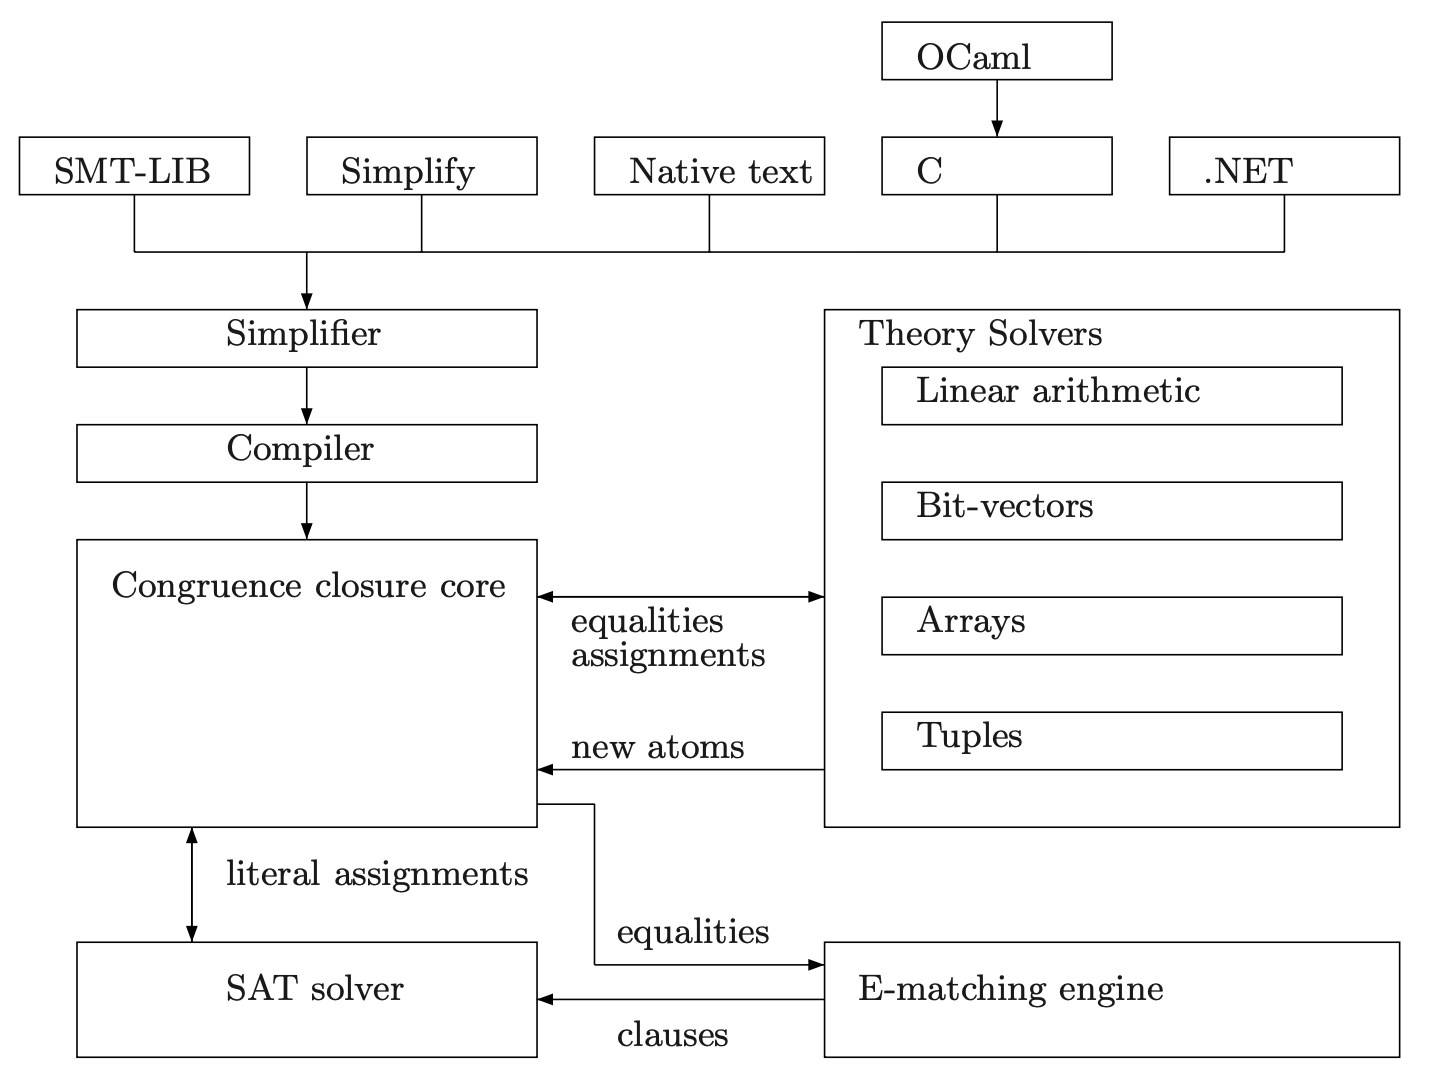
\includegraphics[width=\linewidth]{images/smt-structure}
    \caption{
        Blokový diagram SMT řešiče Z3. \\
        Převzato z článku Z3: An Efficient SMT Solver~\cite{Z3}.
    }
    \label{fig:z3-block-diagram}
\end{figure}

Algoritmus DPLL (Davis-Putnam-Logemann-Loveland) představený roku 1961
je algoritmus pro řešení SAT problémů
založený na rekurzivním prohledávání do hloubky, rozhodování o ohodnocení proměnných a zpětné propagaci (backtracking).
Algoritmus je založen na propagaci jednoduchých důsledků (unit propagation) v případě jednoduchých klauzulí
a rozhodování o ohodnocení proměnných v případě složitějších klauzulí.

Rozšířený algoritmus DPLL(T) zahrnuje teorii T, podporovanou SMT řešičem.
Tento algoritmus se skládá ze dvou částí.
První část je algoritmus DPLL pro SAT, který se stará o generování kandidátních ohodnocení proměnných.
SMT řešič kóduje vlastnosti z teorie T do booleovských proměnných a klauzulí.
Druhá část je SMT řešič dané teorie, který dostává kandidátní ohodnocení proměnných od SAT řešiče a kontroluje logickou konzistenci
v rámci dané teorie.
Tento proces se opakovaně provádí a pokud je nalezena neslučitelnost v SMT teorii,
tak SMT řešič informuje SAT řešič o dané neslužitelnosti pomocí konfliktní klauzule.
Tato klauzule je poté přidána do původní formule a DPLL algoritmus pokračuje v hledání dalšího ohodnocení proměnných
v rozšířené formuli~\cite{DPLLT}.

Následující příklad demonstruje, jakým způsobem SMT řešiče fungují.
Teorie pro tento příklad je lineární celočíselná aritmetika (LIA, Linear Integer Arithmetic).
Vstupní formule pro SMT řešič popisuje tento problém:

\begin{equation*}
    (x \geq 0) \land (x \geq 1 \lor x \leq -1)
\end{equation*}

Tento vstup je nejdříve zakódován do booleovských proměnných a klauzulí.
Konkrétně u tohoto příkladu si SMT řešič zapamatuje mapování

\begin{align*}
    A &= \{ x \geq 0 \} \\
    B &= \{ x \geq 1 \} \\
    C &= \{ x \leq -1 \}
\end{align*}
a vygeneruje formuli pro SAT řešič

\begin{equation*}
    A \land (B \lor C)
\end{equation*}

Tato formule je poté předána SAT řešiči, který se pokusí najít ohodnocení proměnných.
Pomocí jednotkové propagace SAT řešič zjistí, že $A$ musí být pravdivé.
V druhé klauzuli $B \lor C$ se SAT řešič náhodně rozhodne a nastaví $C$ na pravdivé ohodnocení.
Tímto způsobem SAT řešič zjistí, že ohodnocení

\begin{align*}
    A &= \texttt{true} \\
    C &= \texttt{true}
\end{align*}
splňuje danou formuli a přepošle toto kandidátní ohodnocení SMT řešiči.

Pro SMT toto ohodnocení znamená, že musí platit $x \geq 0$ a zároveň $x \leq -1$.
Toto ohodnocení je v rámci teorie LIA neslučitelné, protože $x$ nemůže být zároveň větší než 0 a menší než -1.
SMT řešič tedy informuje SAT řešič o této neslučitelnosti pomocí konfliktní klauzule

\begin{equation*}
    \neg (A \land C) = \neg A \lor \neg C
\end{equation*}
a celá formule pro SAT řešič se tedy změní na

\begin{equation*}
    A \land (B \lor C) \land (\neg A \lor \neg C)
\end{equation*}

Rekurzivním prohledáváním SAT řešič nyní nastaví ohodnocení $B$ na pravdivé,
jelikož by jinak nebylo možné splnit klauzuli $B \lor C$.
Zároveň nastaví $C$ na nepravdivé,
protože je stále $A$ pravdivé a poslední klauzule je splnitelná
pouze pokud je $C$ nastaveno na nepravdu.
A tedy nové kandidátní ohodnocení

\begin{align*}
    A &= \texttt{true} \\
    B &= \texttt{true} \\
    C &= \texttt{false}
\end{align*}
je odesláno pro kontrolu SMT řešiči.

SMT řešic kontroluje pouze pravidivě ohodnocené proměnné $A$ a $B$.
Kombinace těchto proměnných reprezentuje podmínku $x \geq 0$ a $x \geq 1$,
což je v rámci teorie LIA slučitelné.
Jelikož SAT řešič našel ohodnocení proměnných, které splňuje celou formuli
a SMT řešič potvrdil, že toto ohodnocení je slučitelné v rámci dané teorie,
tak lze prohlásit vstupní formuli za splnitelnou v rámci dané teorie.

\section{Standard SMT-LIB}
\label{sec:smt-lib}

SMT-LIB je standardizovaný jazyk pro SMT, který definuje syntaxi a sémantiku pro zápis SMT problémů.
Tento standard byl vyvinut pro usnadnění výzkumu, vývoje a porovnávání různých SMT řešičů.

Od roku 2005 se pravidelně pořádá soutěž SMT-COMP (SMT Competition),
ve které se porovnávají různé SMT řešiče na základě jejich výkonu na různých typech problémů.
Problémy jsou definovány ve formátu SMT-LIB~\cite{SMTCOMP}.

Ukázka~\ref{lst:smt-lib-example} zobrazuje příklad SMT-LIB kódu pro booleovskou formuli

\begin{equation*}
    p \land (p \lor \neg q)
\end{equation*}
kde $p$ a $q$ jsou booleovské proměnné.

\begin{listing}[H]
    \begin{minted}{lisp}
    (set-logic QF_UF)

    (declare-const p Bool)
    (declare-const q Bool)

    (assert (and p (or p (not q))))

    (check-sat)
    (get-model)
    \end{minted}
    \caption{Příklad SMT-LIB kódu pro booleovskou logiku}
    \label{lst:smt-lib-example}
\end{listing}

Pomocí volání funkce \texttt{check-sat} lze zjistit, zdali existuje řešení pro danou formuli.
Pokud ano, SMT-LIB vrátí \texttt{sat}, jinak vrátí \texttt{unsat}.
Pokud je výsledek \texttt{sat}, lze pomocí funkce \texttt{get-model} získat konkrétní hodnoty proměnných, které splňují danou formuli.
Pro tuto formuli byl nalezen model s ohodnocením $p = \texttt{true}$ a $q = \texttt{false}$.
Zvolená teorie je \texttt{QF\_UF} (Quantifier-Free Uninterpreted Functions),
což znamená, že se jedná o logiku bez kvantifikátorů nad neinterpretovanými funkcemi.
Neinterpretované funkce jsou funkce, které nemají žádnou konkrétní interpretaci a jejich význam je dán pouze jejich syntaktickým zápisem.
Konstanty reprezentující proměnné jsou deklarovány pomocí funkce \texttt{declare-const},
což je pouze syntaktický cukr pro neinterpretovanou funkci bez parametrů~\cite{SMTLIB}.

Ukázka~\ref{lst:smt-lib-example-int} zobrazuje příklad SMT-LIB kódu pro celočíselnou aritmetiku.
Konkrétně se jedná o příklad se soustavou dvou rovnic o dvou neznámých.

\begin{align*}
    x + y &= 5 \\
    2x - y &= 4
\end{align*}
kde $x$ a $y$ jsou celočíselné proměnné.

\begin{listing}[H]
    \begin{minted}{lisp}
    (set-logic QF_LIA)

    (declare-const x Int)
    ; syntax sugar for (declare-fun y () Int)
    (declare-const y Int)

    (assert (= (+ x y) 5))
    (assert (= (- (* 2 x) y) 4))

    (check-sat)
    (get-model)
    \end{minted}
    \caption{Příklad SMT-LIB kódu pro celočíselnou aritmetiku}
    \label{lst:smt-lib-example-int}
\end{listing}

Pomocí SMT řešiče lze získat řešení $x = 3$ a $y = 2$.

Pokud bychom měli funkci, která by mohla obsahovat více než jedno řešení,
jako například

\begin{equation*}
    x^2 - 4 = 0
\end{equation*}
mohli bychom interaktivně s SMT řešičem procházet jednotlivá řešení.
Po získání prvního řešení bychom mohli přidat další podmínku, která by vyloučila
první nalezené řešení a pokračovat v hledání dalších řešení.
Tento interaktivní přístup je vhodné naprogramovat, ale výsledné volání SMT řešiče
by vypadalo stejně, jako v následujícím příkladu~\ref{lst:smt-lib-example-sqrt}.

\begin{listing}[H]
    \begin{minted}{lisp}
    (set-logic QF_LIA)

    (declare-const x Int)

    (assert (= (- (* x x) 4) 0))

    (check-sat)
    (get-model)

    (assert (not (= x 2)))

    (check-sat)
    (get-model)

    (assert (not (= x -2)))

    (check-sat)
    \end{minted}
    \caption{Příklad SMT-LIB kódu pro hledání více řešení}
    \label{lst:smt-lib-example-sqrt}
\end{listing}

Tímto postupem nám SMT řešič postupně oznámí dvakrát výsledek \texttt{sat} s modelem pro proměnnou $x$ s hodnotami $2$ a $-2$.
Nakonec oznámí výsledek \texttt{unsat}, což znamená, že neexistuje další řešení a program by měl skončit.


\chapter{Hoareova logika}
\label{ch:hoareova-logika}

Formální systém označovaný jako Hoareova logika byl navržen a popsán
britským matematikem a informatikem C. A. R. Hoarem v roce 1969~\cite{Hoare1969}.
Jedná se o formální systém pro popis a analýzu počítačových programů,
který pro důkaz správnosti programů používá předpoklady (preconditions) a následky (postconditions).

Program popisujeme pomocí Hoareovy trojice

\begin{equation*}
    \{P\} \  Q \  \{R\},
\end{equation*}
kde $P$ jsou předpoklady popisující stav systému před provedením programu,
$Q$ je daný program (příkaz či sekvence příkazů)
a $R$ jsou následky, které popisují stav systému po provedení tohoto programu.
Takto popsaný systém čteme následovně:
\uv{Při splněných předpokladech $P$ budou po provedení programu $Q$ zaručeny následky $R$}.

Hoare v roce 1969 definoval trojici jako $P \ \{ Q \} \  R$,
ale v současnosti se častěji setkáme se zápisem $\{ P \} \  Q \ \{ R \}$.

Předpoklady a následky jsou vyjádřeny jako logické formule,
které popisují vlastnosti proměnných programu v určitém okamžiku.
Následující příklad reprezentuje program, který předpokládá na vstupu nezápornou hodnotu v proměnné $x$
a po provedení programu $Q$ bude zajištěno, že hodnota proměnné $x$ bude kladná (ostře větší než 0).

\begin{equation*}
    \{ x \geq 0 \} \  x \coloneqq x + 1 \  \{ x > 0 \}
\end{equation*}

Předpoklad může být také prázdný, což znamená, že program nevyžaduje žádné speciální podmínky pro spuštění
a formálně tuto situci lze zapsat jako $\{ true \} \  Q \  \{ R \}$.
Pokud je předpoklad prázdný, předpokládáme, že program může být spuštěn
v libovolném stavu systému nebo s libovolnými hodnotami proměnných.
Takový program může vypadat následovně:

\begin{equation*}
    \{ true \} \  x \coloneqq 10 \  \{ x > 0 \}
\end{equation*}

\section{Axiom přiřazení}
\label{sec:hoare-axiom-prirazeni}

Axiom přiřazení je základním pravidlem Hoareovy logiky a nedílnou součástí každého počítačového programu.
Přiřazení je operace obecně zapsaná ve tvaru

\begin{equation*}
    x \coloneqq f,
\end{equation*}
kde $x$ je proměnná a $f$ je výraz bez vedlejších efektů (side effect),
který ale může obsahovat proměnnou $x$, například $x \coloneqq x + 1$.

Chceme zajistit, že jakékoli tvrzení $T$ platné o $f$
je také platné o hodnotě proměnné $x$ po provedení přiřazení.
Označíme si $T[x \leftarrow f]$ tvrzení $T$ ve kterém výskyt proměnné $x$ nahradíme výrazem $f$ (substituce).

Poté můžeme definovat axiom přiřazení jako

\begin{equation*}
    \{ T[x \leftarrow f] \} \  x \coloneqq f \  \{ T \}.
\end{equation*}

Tento zápis říká, že pokud je pravdivé tvrzení $T$, ve kterém
je výskyt proměnné $x$ nahrazen výrazem $f$, pak po provedení přiřazení
je tvrzení $T$ pravdivé také pro proměnnou $x$.
Jedná se tedy o šablonu (schéma) axiomu,
kterou lze použít pro libovolné tvrzení $T$, proměnnou $x$ a výraz $f$.

\section{Pravidlo důsledku}
\label{sec:hoare-pravidlo-dusledku}

Pravidlo důsledku (rule of consequence) je metoda umožnující
tvorbu nových logických tvrzení z již existujících a dokázaných tvrzení.
Základní aplikací této metody je pravidlo \textbf{rozšíření předpokladu}
a pravidlo \textbf{zůžení následku}.
Předpokládejme platnosti $\{ P \} \  Q \  \{ R \}$.

Máme-li rozšířený předpoklad $P'$, pro který platí

\begin{equation*}
    P' \implies P
\end{equation*}
můžeme říci, že

\begin{equation*}
    \{ P' \} \  Q \  \{ R \}
\end{equation*}
je také platné tvrzení.

Máme-li zúžený následek $R'$ následku $R$, pro který platí

\begin{equation*}
    R \implies R'
\end{equation*}
můžeme říci, že $\{ P \} \  Q \  \{ R' \}$ je také platné tvrzení.

\section{Pravidlo skládání}
\label{sec:hoare-pravidlo-skladani}

Pravidlo skládání (rule of composition) je pravidlo, které umožňuje
skládat více příkazů do jednoho složeného příkazu a používat jeje v Hoareově logice.

Máme-li dva příkazy $Q_1$ a $Q_2$, které splňují následující tvrzení

\begin{equation*}
    \{ P_1 \} \  Q_1 \  \{ R_1 \}
\end{equation*}
a

\begin{equation*}
    \{ R_1 \} \  Q_2 \  \{ R_2 \}
\end{equation*}
můžeme říci, že složený příkaz $Q_1; Q_2$ splňuje následující tvrzení

\begin{equation*}
    \{ P_1 \} \  Q_1; Q_2 \  \{ R_2 \}
\end{equation*}
kde $;$ je operátor sekvence příkazů, který říká, že příkaz $Q_1$ bude proveden před příkazem $Q_2$.

Toto pravidlo umožňuje vytvářet složitější příkazy z několika jednodušších příkazů.
Zároveň je možné rozmyslet, že na sekvenci příkazů $Q_1, Q_2, \ldots, Q_n$
lze aplikovat stejné pravidlo skládání, které jsme použili pro dva příkazy
pomocí asociativity operátoru $;$ a závorek. A tedy platí, že

\begin{equation*}
    \{ P \} \  Q_1; Q_2; \  \ldots ; Q_n \  \{ R \}
\end{equation*}
je ekvivalentní s

\begin{equation*}
    \{ P \} \  (Q_1; (Q_2; \  \ldots (Q_{n-1}; Q_n))) \  \{ R \}
\end{equation*}

\section{Pravidlo iterace}
\label{sec:hoare-pravidlo-iterace}

Základním stavebním blokem počítačového programu je cyklus.
V Hoareově logice je cyklus reprezentován pomocí pravidla iterace (rule of iteration)
a využívá $while$ cyklus, který je v programovacích jazycích běžně dostupný a je definován následovně:

\begin{equation*}
    \textbf{while} \  B \  \textbf{do} \  Q
\end{equation*}
kde $Q$ je tělo cyklu, které se v každé iteraci provádí, dokud je podmínka $B$ pravdivá.

Dále definujeme invariant cyklu $I$, který nám pomůže
při rozhodování o správnost cyklu a bude popisovat následky provedení cyklu.
Invariant cyklu je logické tvrzení, které musí být pravdivé před vstupem do cyklu,
po ukončení každé iterace cyklu a tedy i po ukončení cyklu.

Formálně můžeme zapsat podmínky pro invariant cyklu $I$ jako

\begin{equation*}
    I \land (\{ B \} \  Q \  \{ I \})
\end{equation*}

První část konjunkce popisuje, že invariant cyklu musí být pravdivý před vstupem do cyklu.
Druhá část konjunkce popisuje, že invariant cyklu musí být pravdivý po provedení těla cyklu $Q$,
pokud se cyklus spustil (podmínka $B$ byla pravdivá).

\begin{remark}
    Invariant cyklu je nezávislý na počtu provedených iterací.
\end{remark}

Pokud cyklus neprovedl žádnou iteraci a zároveň máme zaručeno,
že invariant cyklu $I$ byl pravdivý před vstupem do cyklu,
triviálně platí, že invariant cyklu $I$ je pravdivý i po ukončení cyklu.
Zároveň platí, že cyklus se neprovedl, protože podmínka $B$ byla nepravdivá.

Pokud cyklus provedl alespoň jednu iteraci a zároveň máme zaručeno,
že invariant cyklu $I$ je pravdivý po ukončení těla cyklu $Q$,
znamená to, že invariant cyklu $I$ je pravdivý i po ukončení poslední iterace cyklu.
Zároven platí, že podmínka $B$ je po ukončení cyklu nepravdivá, jinak by cyklus pokračoval v provádění další iterace.

Formálně lze tedy konstrukci $while$ cyklu pomocí Hoareovy logiky zapsat jako

\begin{equation*}
    I \land \{ B \} \  Q \  \{ I \} \implies \{ I \} \  \textbf{while} \  B \  \textbf{do} \  Q \  \{ \neg B \land I \}
\end{equation*}

\chapter{Metoda nejslabšího předpokladu}
\label{ch:metoda-nejslabsiho-predpokladu}

Metoda nejslabšího předpokladu (weakest precondition, WP) je metoda,
používaná k algoritmickému dokazování správnosti programů pomocí Hoareovy logiky.
Formálně tuto metodu popsal E. W. Dijkstra v roce 1975 a navazuje na práci Hoareho~\cite{Dijkstra1975}.

Připomeneme, že Hoareova trojice je trojice $ \{ P \} \ Q \ \{ R \} $,
kde $P$ je předpoklad, $Q$ je příkaz a $R$ je následek.
Předpoklad $P$ je logický výraz, který musí být pravdivý před provedením příkazu $Q$.
Metoda nejslabšího předpokladu se snaží najít nejslabší předpoklad $WP$, pro který platí

\begin{equation*}
    \{ WP \} \ Q \ \{ R \}
\end{equation*}

a zároveň pro každý jiný předpoklad $P$, pro který by platilo, že

\begin{equation*}
    \{ P \} \ Q \ \{ R \}
\end{equation*}

musí také platit, že

\begin{equation*}
    P \implies WP
\end{equation*}

Tedy, že $WP$ je nejslabší předpoklad pro příkaz $Q$ a následek $R$.

\begin{remark}
    Nejslabší předpoklad $WP$ je (logicky) unikátní pro daný příkaz $Q$ a následek $R$.
\end{remark}

Pokud by existoval jiný kandidát $WP'$ pro nejslabší předpoklad,
poté z definice platí, že

\begin{equation*}
    WP' \implies WP
\end{equation*}

a také, že

\begin{equation*}
    WP \implies WP'
\end{equation*}

Tedy musí platit, že $WP$ a $WP'$ jsou (logicky) ekvivalentní.

Nejslabší předpoklad $WP$ definujeme pomocí transformační funkce $wp$
s parametry $Q$ a $R$ následovně:

\begin{equation*}
    WP = wp(Q, R)
\end{equation*}

Následující kapitoly představují základní pravidla pro algoritmický výpočet nejslabšího předpokladu.
Výpočet začíná vždy od následku $R$ a postupně (od konce k začátku)
analyzuje příkazy $Q_n, Q_{n-1}, \cdots, Q_1$ a aplikuje na ně specifická pravidla.
Výsledkem je nejslabší předpoklad $WP$ pro sekvenci příkazů $Q_1; Q_2; \cdots; Q_n$,
který následně použijeme pro formální důkaz správnosti programu.

\section{Pravidlo přiřazení}
\label{sec:pravidlo-prirazeni}

Výpočet nejslabšího předpokladu pro přiřazení proměnné $x$ hodnoty $E$ je
definován následovně:

\begin{equation*}
    wp(x \coloneqq E, R) = R[x \mapsto E]
\end{equation*}

kde $R[x \mapsto E]$ je substituce výsktytu proměnné $x$ hodnotou $E$ v $R$.

Například pro příkaz $x \coloneqq x + 3$ a následek $x > 0$ dostáváme:

\begin{align*}
    wp(x \coloneqq x + 3, x > 0) & = \\
                                 & = x + 3 > 0 \\
                                 & = x > -3
\end{align*}

Nejslabší předpoklad pro příkaz $x \coloneqq x + 3$, který zaručuje, že
následek $x > 0$ bude pravdivý, je tedy $x > -3$.

\section{Pravidlo sekvence}
\label{sec:pravidlo-sekvence}

Pravidlo sekvence napomáhá k určení nejslabšího předpokladu pro sekvenci příkazů.
Máme-li dva příkazy $Q_1$ a $Q_2$, které splňují následující tvrzení

\begin{equation*}
    \{ P_1 \} \  Q_1 \  \{ R_1 \}
\end{equation*}

a

\begin{equation*}
    \{ R_1 \} \  Q_2 \  \{ R_2 \}
\end{equation*}

můžeme říci, že nejslabší předpoklad pro sekvenci příkazů $Q_1; Q_2$ je

\begin{equation*}
    wp(Q_1; Q_2, R) = wp(Q_1, wp(Q_2, R))
\end{equation*}

Podobně jako v pravidle skládání u Hoareovy logiky z kapitoly~\ref{sec:hoare-pravidlo-skladani}
můžeme rozmyslet výpočet nejslabšího předpokladu pro sekvenci příkazů $Q_1, Q_2, \cdots, Q_n$
pomocí asociativity operátoru $;$ a rekurzivního výpočtu nejslabšího předpokladu.

Například pro příkaz $x \coloneqq x + 3; y \coloneqq x + 2$ a následek $y > 0$ dostáváme:

\begin{align*}
    wp(x \coloneqq x + 3; y \coloneqq x + 2, y > 0) & = \\
                                                     & = wp(x \coloneqq x + 3, wp(y \coloneqq x + 2, y > 0)) \\
                                                     & = wp(x \coloneqq x + 3, x + 2 > 0) \\
                                                     & = x + 3 + 2 > 0 \\
                                                     & = x > -5
\end{align*}

Nejslabší předpoklad pro příkaz $x \coloneqq x + 3; y \coloneqq x + 2$, který zaručuje, že
následek $y > 0$ bude pravdivý, je tedy $x > -5$.

\section{Pravidlo podmínky}
\label{sec:pravidlo-podminky}

Pravidlo podmínky popisuje výpočet nejslabšího předpokladu pro podmínkový příkaz ve tvaru:

\begin{equation*}
    \textbf{if} \ B \ \textbf{then} \ Q_T \ \textbf{else} \ Q_F
\end{equation*}

kde $B$ je podmínka, $Q_T$ je příkaz, který se provede, pokud je podmínka $B$ pravdivá,
a $Q_F$ je příkaz, který se provede, pokud je podmínka $B$ nepravdivá.

Pravidlo podmínky je definováno následovně:

\begin{align*}
    wp(\textbf{if} & \ B \ \textbf{then} \ Q_T \ \textbf{else} \ Q_F, R) = \\
                   & = (B \implies wp(Q_T, R)) \land (\neg B \implies wp(Q_F, R))
\end{align*}

Tedy nejslabší předpoklad pro podmínkový příkaz je logická konjunkce dvou implikací.
Nejslabší předpoklad totiž musí zahrnout oba možné stavy podmínky $B$, případ, kdy je $B$ pravdivá ale také případ, kdy je $B$ nepravdivá.

Pokud je podmínka $B$ pravdivá, použijeme nejslabší předpoklad pro příkaz $Q_T$, tedy $wp(Q_T, R)$.
Pokud není pravdivá ($\neg B$), použijeme nejslabší předpoklad pro příkaz $Q_F$, tedy $wp(Q_F, R)$.

Například pro příkaz $if \ x > 0 \ then \ y \coloneqq x + 3 \ else \ y \coloneqq x - 3$
a následek $y > 0$ dostáváme:

\begin{align*}
    wp(if & \ x > 0 \ then \ y \coloneqq x + 3 \ else \ y \coloneqq x - 3, y > 0) = \\
          & = (x > 0 \implies wp(y \coloneqq x + 3, y > 0)) \land (\neg (x > 0) \implies wp(y \coloneqq x - 3, y > 0)) \\
          & = (x > 0 \implies x + 3 > 0) \land (\neg (x > 0) \implies x - 3 > 0) \\
          & = (x > 0 \implies x > -3) \land (\neg (x > 0) \implies x > 3)
\end{align*}

Použitím pravidla implikace

\begin{align*}
    (P \implies A) \land (\neg P \implies B) & \iff (P \land A) \lor (\neg P \land B)
\end{align*}

můžeme původní výraz zjednodušit následovně:

\begin{align*}
    (x > 0 & \implies x > -3) \land (\neg (x > 0) \implies x > 3) = \\
           & = (x > 0 \land x > -3) \lor (\neg (x > 0) \land x > 3) \\
           & = (x > 0 \land x > -3) \lor (x \leq 0 \land x > 3) \\
           & = (x > 0 \land x > -3) \lor (false) \\
           & = x > 0 \land x > -3 \\
           & = x > -3
\end{align*}

Výpočet nejslabšího předpokladu pro příkaz $if \ x > 0 \ then \ y \coloneqq x + 3 \ else \ y \coloneqq x - 3$,
který zaručuje, že následek $y > 0$ bude pravdivý, je tedy $x > -3$.
Poslední zjednodušení je možné provést, protože $x > 0$ je silnější předpoklad než $x > -3$,
platí že $x > 0 \implies x > -3$.

Zároveň jsme při výpočtu zjistili, že negativní část ($else$) podmínky nemá vliv na výpočet nejslabšího předpokladu,
protože neexistuje žádný předpoklad, který by v případě, že $x \leq 0$ a $y \coloneqq x - 3$, zaručoval, že $y > 0$.

% TODO: navazat treba na Frama-c, ze pokud dokazeme takovyto priklad, tak vsechny
% TODO: i nelogicke priklady po tom jsou podminene pravdive, nehlede na to, ze
% TODO: ze nemaji treba splnitelnost = assert \false

\chapter{Frama-C}
\label{ch:frama-c}

V oblasti formální verifikace softwaru hrají významnou roli nástroje umožňující
statickou analýzu zdrojového kódu a deduktivní dokazování správnosti těchto programů.
Mezi ustálené platformy zaměřené na analýzu programů napsaných v jazyce C patří prostředí Frama\mbox{-}C,
které poskytuje užitečné nástroje a možnost rozšíření o moduly a pluginy~\cite{FCKernelMaroneze2024}.
Frama\mbox{-}C je open-source nástroj, který byl vyvinut na výzkumném ústavu CEA-LIST (Commissariat à l'Énergie Atomique et aux Énergies Alternatives)
a první verze byla vydána v roce 2008.

Jádro Frama\mbox{-}C je napsáno v jazyce OCaml a je postaveno jako modulární framework
navržený s cílem usnadnit aplikaci pokročilých technik formální analýzy nad programy v jazyce C
pomocí integrace různých analytických nástrojů ve formě pluginů~\cite{FCPluginDevSignoles2024}.
Některé z těchto pluginů jsou obsaženy přímo v jádře Frama\mbox{-}C, zatímco další jsou dostupné jako externí moduly.
Moduly obsažené v jádře Frama\mbox{-}C zahrnují například deduktivní analyzátor WP (Weakest Precondition)
založený na teoretickém základu popsaném v kapitole~\ref{ch:metoda-nejslabsiho-predpokladu},
RTE (Run-Time Error) pro detekci chyb při běhu programu, který si představíme v kapitole~\ref{sec:frama-c-rte},
nebo například EVA (Evolving Value Analysis) pro analýzu hodnot proměnných v průběhu vykonávání programu.

Klíčovým prvkem Frama\mbox{-}C je definice a podpora specifikačního jazyka ACSL (ANSI/ISO C Specification Language),
který umožňuje uživatelům vyjadřovat vlastnosti a specifikace programů v jazyce C pomocí specifikačních komentářů.
Tyto komentáře anotují kód a poskytují informace pro statickou analýzu a deduktivní dokazování.
Návrh a implementace ACSL byly inspirovány podobným standardem JML (Java Modeling Language) pro jazyk Java~\cite{ACSLSpec}.
Jazyk ACLS bude podrobněji představen v kapitole~\ref{sec:acsl}.

Prostředí Frama\mbox{-}C je distribuováno jako program pro příkazový řádek a také jako grafické uživatelské rozhraní (GUI),
které poskytuje uživatelsky přívětivé prostředí pro interakci s celým ekosystémem Frama\mbox{-}C a hlavně s nainstalovanými pluginy.
Grafické prostředí je dostupné hlavně pro operační systémy Linux a Windows.
Pro uživatele operačního systému macOS je k dispozici pouze příkazová řádka.

Distibuce Frama\mbox{-}C obsahuje mimo jiné také Docker image,
který obsahuje všechny potřebné závislosti pro běh Frama\mbox{-}C\@.
Součástí image jsou základní pluginy jako například WP, EVA a RTE
společně s SMT řešičemi Alt-Ergo, CVC4 a Z3.
Lze využít také GUI variantu image, který se od základního liší
nainstalovaným grafickým uživatelským rozhraním (GUI) Frama\mbox{-}C,
minimalistickým desktopovým prostředím a VNC serverem.
Na tento VNC server se lze připojit pomocí webového prohlížeče
a lze tedy používat GUI například i na macOS nebo jiných operačních systémech
bez nutnosti speciálního nastavení nebo instalace~\cite{FCDockerGUIMaroneze2021}.

% TODO: převádí -> převede? jaký čas/rod? (spíš převádí)

Frama\mbox{-}C před spuštěním analýzy převádí zdrojový kód do mezi-interpretace (intermediate representation)
nazývané \texttt{CIL} (C Intermediate Language)~\cite{BlanchardACSL2024}.
Frama\mbox{-}C používá vlastní verzi \texttt{CIL}, která je založena na původní verzi, kterou vytvořil George Necula~\cite{Necula2002CIL}.
Od roku 2016 tato původní verze již není udržována, ale Frama\mbox{-}C stále podporuje vlastní verzi.
Vlastní předzpracování a použití mezi-interpretace umožňuje Frama\mbox{-}C
analyzovat zdrojový kód efektivněji a nainstalované pluginy mohou pracovat
s touto abstraktní reprezentací, upravovat ji nebo dokonce transformovat~\cite{FCKernelMaroneze2024}.

Základní pluginy Frama\mbox{-}C jsou součástí distribuce a jsou dostupné zdarma.
Je vhodné zmínit například plugin Frama\mbox{-}Clang, jehož cílem je
přidat podporu programovacího jazku C\texttt{++} do Frama\mbox{-}C\@.
Frama\mbox{-}Clang je aktuálně ve vývoji a je dostupný pro experimentování a testování,
ale není doporučeno jej používat pro produkční nasazení~\cite{framaclang}.

Jiné pluginy mohou být dostupné pod jinými licencemi nebo jako komerční produkty.
Jedním z proprietárních pluginů je například plugin pro generování protipříkladů
(counterexamples) pro Frama\mbox{-}C\@.
Tato funkcionalita je i s tímto pluginem dostupná pouze pro SMT řešič Alt-Ergo,
což může být nevhodné pro uživatele, kteří preferují jiné SMT řešiče nebo na úlohy,
které nejsou vhodné pro Alt-Ergo~\cite{framacounterexamples}.

\section{ACSL (ANSI/ISO C Specification Language)}
\label{sec:acsl}

ACLS je specifikační jazyk pro jazyk C, který umožňuje uživatelům
vyjadřovat vlastnosti a specifikace programů pomocí anotací v podobě speciálních komentářů ve zdrojovém kódu.

Anotace lze zapsat jako jednořádkový komentář \texttt{//@ ...} nebo víceřádkový komentář \texttt{/*@ ... */} umístěný přímo ve zdrojovém kódu.
Ukázka~\ref{list:acsl-example} zobrazuje příklad zdrojového kódu ve kterém nalezneme obě varianty anotací.

\begin{listing}[H]
    \begin{minted}{C}
    /*@
      requires x > 0;
      assigns \result;
      ensures \result == x + 2;
    */
    int increment(int x) {
      x = x + 1;
      //@ assert x > 1;
      return x + 1;
    }
    \end{minted}
    \caption{Ukázka anotací v jazyce C pomocí ACSL}
    \label{list:acsl-example}
\end{listing}

V návaznosti na kapitolu~\ref{ch:metoda-nejslabsiho-predpokladu},
ve které byla teoreticky popsána metoda nejslabšího předpokladu,
nyní navážeme a představíme ACSL anotace umožňující zápis specifikací a vlastností programů,
které společně se zdrojovým kódem zpracovává WP (Weakest Precondition) plugin Frama\mbox{-}C\@.

Ukázka~\ref{list:acsl-example} představila funkci \texttt{increment},
která definuje předpoklad a následek pomocí klíčových slov \texttt{requires} a \texttt{ensures}.
Zjednodušená Hoareova trojice pro tuto funkci by vypadala následovně:

\begin{equation*}
    \{ x > 0 \} \ (x = x + 1; \textbf{return} \  x + 1) \ \{ \textbf{result} == x + 2 \}
\end{equation*}

Anotace \texttt{requires} se používá k vyjádření předpokladů
u kterých předpokládáme, že jsou splněny před provedením funkce.
Syntakticky je možné použít \texttt{requires} pouze v kontraktech funkcí.

Anotace \texttt{ensures} se používá k vyjádření následků,
které budou platit, za předpokladu úspěšného provedení důkazu, po provedení funkce.
Syntakticky je možné použít \texttt{ensures} pouze v kontraktech funkcí.

Anotace \texttt{requires} a \texttt{ensures}
jsou přímou aplikací Hoareovy logiky na funkcích v jazyce C\@.
Předpoklady z Hoareovy logiky jsou vyjádřeny pomocí klauzule \texttt{requires},
následky pomocí klauzule \texttt{ensures} a příkaz (program) je vyjádřen jako tělo funkce.

Frama\mbox{-}C převádí kód napsaný v jazyce C společně s ACSL anotacemi do formálního jazyka WhyML,
který je součástí platformy Why3 a poskytuje podporu pro specifikaci vlastností programů
a následného ověření pomocí externích dokazovacích nástrojů~\cite{why3web}.
Plaforma Why3 slouží jako univerzální mezi-vrstva mezi popisem programu v jazyce WhyML a různými SMT řešiči
jako jsou například Alt-Ergo, CVC4 a Z3~\cite{boogie11why3}.
Cílem Why3 je poskytnout jednotné rozhraní pro specifikaci a verifikaci programů
a náslédně automaticky generovat formální důkazy pomocí různých SMT řešičů bez nutnosti přepisovat kód pro každý SMT řešič zvlášť.
Why3 je zakomponován do několika nástrojů pro formální verifikaci,
jako je například Frama\mbox{-}C pro jazyk C~\cite{BlanchardACSL2024},
Krakatoa pro jazyk Java~\cite{KrakatoaWhy} nebo například projekt Easycrypt,
který se zaměřuje na formální verifikaci kryptografických protokolů~\cite{why3web}.

Jednou nevýhodou platformy Why3 je,
že nepodporuje všechny nejnovější verze SMT řešičů.
Následující tabulka~\ref{tab:why3-smt-verze}
zobrazuje podporované verze SMT řešičů v platformě Why3 společně s jejich nejnovějšími verzemi.

\begin{table}[H]
    \centering
    \begin{tabular}{|c|c|c|}
        \hline
        SMT řešič & Podporovaná verze & Nejnovější verze \\
        \hline
        Alt-Ergo  & 2.5.4             & 2.6.1            \\
        CVC4      & 1.8               & 1.8              \\
        CVC5      & 1.0.9             & 1.2.1            \\
        Z3        & 4.8.17            & 4.14.1           \\
        \hline
    \end{tabular}
    \caption{Podporované verze SMT řešičů v platformě Why3}
    \label{tab:why3-smt-verze}
\end{table}

% TODO: jsou ..použity.. -> používá?

Frama\mbox{-}C definuje několik základních axiomů, lemmat, predikátů, funkcí a typů,
které jsou použity v rámci generování WhyML kódu~\cite{FCGitWhy} a
některé ukázky v následujících kapitolách budou pro úplnost doplněny o tyto definice jazyce WhyML\@.

% TODO: je to v teto sekci?

\subsection{Obecný a existenční kvantifikátor}
\label{subsec:anotace-kvantifikatory}

% TODO: uživatelům/programátorům?

Obecný kvantifikátor \texttt{\textbackslash forall} a existenční kvantifikátor \texttt{\textbackslash exists}
umožňují uživatelům vyjadřovat vlastnosti proměnných a paměťových oblastí.
Jejich použití nejčastěji nalezneme v kontraktech funkcí,
kde kvantifikátory pomáhají vyjádřit vlastnosti o parametrech funkcí nebo návratových hodnotách.

% TODO: říká -> specifikuje...?

Příklad~\ref{list:acsl-forall} zobrazuje použití obecného kvantifikátoru,
který se používá k vyjádření vlastnosti, která musí být splněna pro všechny hodnoty.
Zde je definována vlastnost prvků v poli celých čísel \texttt{arr} o velikosti \texttt{n},
která specifikuje, že pro každé $i$ v intervalu $[0, n)$ platí,
že hodnota $arr[i]$ (prvek pole) je větší nebo rovna nule (pole obsahuje pouze nezáporné hodnoty).

Predikát \texttt{\textbackslash valid} zajišťuje,
že ukazatel \texttt{arr} ukazuje na platnou paměťovou oblast
a \texttt{(0..n-1)} specifikuje rozsah platných indexů tohoto pole.
Platnost ukazatelů popisuje kapitola~\ref{sec:ukazatele-a-pametove-bloky}.

\begin{listing}[H]
    \begin{minted}{C}
    /*@
      requires \valid(arr + (0..n-1));
      requires n > 0;

      requires
        \forall integer i;
          0 <= i < n
            ==> 0 <= arr[i];
    */
    int find_min(int *arr, int n) {
    }
    \end{minted}
    \caption{Ukázka obecného kvantifikátorů v ACSL}
    \label{list:acsl-forall}
\end{listing}

% TODO: ukazuje -> zobrazuje

Použití existenčního kvantifikátoru \texttt{\textbackslash exists} je podobné,
ale místo toho, aby vyžadoval splnění vlastnosti pro všechny hodnoty,
umožňuje vyjádřit, že existuje alespoň jeden prvek, pro který je daná vlastnost splněna.
Příklad~\ref{list:acsl-exists} zobrazuje anotaci funkce pro hledání minimální hodnoty v poli celých (nezáporných) čísel.
Anotace specifikuje, že výsledná hodnota funkce je hodnota některého prvku v poli.

\begin{listing}[H]
    \begin{minted}{C}
    /*@
      ...
      ensures
        \exists integer i;
          0 <= i < n
            ==> arr[i] == \result;
    */
    int find_min(int *arr, int n) {
    }
    \end{minted}
    \caption{Ukázka existenčního kvantifikátoru v ACSL}
    \label{list:acsl-exists}
\end{listing}

Nicméně tato anotace sama o sobě specifikuje pouze to, že existuje prvek v poli,
který má stejnou hodnotu jako návratová hodnota funkce.
Tato anotace by byla splnitelná i jednoduchým kódem, který vrací první prvek pole (například \texttt{return arr[0]}).
Jelikož je zajištěno, že $n$ je alespoň 1 (\texttt{requires~n~>~0}),
tak je tento program korektní a splňuje kontrakt funkce.

% TODO: je zobrazeno -> zobrazuje?
% TODO: trpný rod/prítomný

% TODO: je zobrazeno -> zobrazuje

Kontrakt je tedy nedostatečný, protože nespecifikuje vlastnost,
že by tento prvek byl doopravdy minimální.
Pokud bychom chtěli vyjádřit, že tento prvek je minimální,
museli bychom přidat kombinaci obecného a existenčního kvantifikátoru,
jak je zobrazeno v ukázce~\ref{list:acsl-exists-forall},
která nám umožňuje vyjádřit vlastnost, že existuje prvek v poli,
jehož hodnota je rovna výsledku funkce a zároveň splňuje vlastnost,
že je minimální vůči všem ostatním prvkům v poli.

\begin{listing}[H]
    \begin{minted}{C}
    /*@
      ...

      ensures
        \exists integer i;
          0 <= i < n
            ==> arr[i] == \result
            && \forall integer j;
              0 <= j < n
                ==> \result <= arr[j];
    */
    int find_min(int *arr, int n) {
    }
    \end{minted}
    \caption{Ukázka kombinace obecného a existenčního kvantifikátoru v ACSL}
    \label{list:acsl-exists-forall}
\end{listing}

Pro dokončení důkazu funkce \texttt{find\_min} je nutné přidat do kódu cyklus,
který bude procházet polem a hledat minimální prvek.
Anotace a důkazy cyklů popisuje následující kapitola~\ref{subsec:acsl-cykly},
na jejímž konci dokončíme důkaz funkce \texttt{find\_min}.

\subsection{Cykly}
\label{subsec:acsl-cykly}

Cykly v jazyce C jsou reprezentovány pomocí konstrukcí \texttt{for}, \texttt{while} a nebo \texttt{do-while}.
Frama\mbox{-}C v rámci předzpracování kódu převádí tyto konstrukce pouze na konstrukci \texttt{while}.
Následující ukázky~\ref{list:for-transform-while} a~\ref{list:do-while-transform-while}
ukazují ekvivalentní zápis cyklu \texttt{for} a \texttt{do-while} pomocí cyklu \texttt{while}.
Stejnou transformace cyklů provádí Frama\mbox{-}C automaticky během předzpracování zdrojového kódu.

\begin{listing}[H]
    \begin{minted}{C}
    for (init; condition; increment) {
      body;
    }

    // ekvivalentní zápis

    init;
    while (condition) {
      body;
      increment;
    }
    \end{minted}
    \caption{Ekvivalentní zápis cyklu \texttt{for} pomocí \texttt{while}}
    \label{list:for-transform-while}
\end{listing}

\begin{listing}[H]
    \begin{minted}{C}
    do {
      body;
    } while (condition);

    // ekvivalentní zápis

    while (1) {
      body;
      if (!condition) break;
    }
    \end{minted}
    \caption{Ekvivalentní zápis cyklu \texttt{do-while} pomocí \texttt{while}}
    \label{list:do-while-transform-while}
\end{listing}

Tvorba důkazů pro cykly je složitější než pouze pro sekvenci příkazů.
Stejně jako v Hoareově logice je v ACSL nutné pro správné důkazy cyklů definovat invarianty cyklu (\texttt{loop invariant}).
Invariant je vlastnost, která musí být splněna před spuštěním cyklu,
na konci každé iterace cyklu a také po ukončení cyklu.
Pokud invariant nespecifikujeme, jako například v ukázce~\ref{list:loop-no-invariant},
poté pomocí metody nejslabšího předpokladu nelze prokázat,
že cyklus skončí a že proměnná \texttt{n} bude mít požadovanou hodnotu 0.

\begin{listing}[H]
    \begin{minted}{C}
    /*@
      requires n >= 0;
    */
    void loop_invariant(int n) {
      while (n > 0) {
        n--;
      }
      //@ assert n == 0;
    }
    \end{minted}
    \caption{Ukázka cyklu bez invariantu}
    \label{list:loop-no-invariant}
\end{listing}

\begin{listing}[H]
    \begin{minted}{console}
    frama-c -wp -wp-prover alt-ergo,cvc4,z3 \
      -wp-no-let -wp-print no-loop-invariant.c
    \end{minted}
    \caption{Příkaz pro spuštění analýzy cyklu bez invariantu pomocí třech SMT řešičů}
    \label{list:loop-no-invariant-command}
\end{listing}

\begin{listing}[H]
    \begin{minted}{text}
    Goal Termination-condition (generated) in 'loop_invariant':
    Loop termination at line 5
    Assume {
      Type: is_sint32(n).
      (* Pre-condition *)
      Have: 0 <= n.
      (* Pre-condition *)
      Have: 0 <= n.
    }
    Prove: false.
    Prover Alt-Ergo 2.5.3 returns Timeout (2s)
    Prover CVC4 1.8 returns Unknown
    Prover Z3 4.8.12 returns Timeout (2s)

    ---

    Goal Assertion (file no-loop-invariant.c, line 8):
    Assume {
      Type: is_sint32(n) /\ is_sint32(n_1) /\ is_sint32(n_2).
      (* Pre-condition *)
      Have: 0 <= n_2.
      (* Pre-condition *)
      Have: 0 <= n_2.
      (* Else *)
      Have: n_1 <= 0.
      Have: n_1 = n.
    }
    Prove: n = 0.
    Prover Alt-Ergo 2.5.3 returns Timeout (2s)
    Prover CVC4 1.8 returns Unknown
    Prover Z3 4.8.12 returns Timeout (2s)
    \end{minted}
    \caption{Výstup analýzy cyklu bez invariantu}
    \label{list:loop-no-invariant-output}
\end{listing}

Spuštěním příkazu~\ref{list:loop-no-invariant-command} získáme výsledek analýzy~\ref{list:loop-no-invariant-output},
který ukazuje, že proběhl pokus o dokázání dvou vlastností.
První vlastnost je automaticky generovaná podmínka konečnosti cyklu, kterou uživatel musí vyplnit.
Konečnost cyklů bude popsána na konci této kapitoly.
Druhá vlastnost je naše očekávaná vlastnost (\texttt{assert n == 0}),
kterou nemohl zádný z použitých SMT řešičů dokázat.
Jediná informace, kterou SMT řešiče o proměnné \texttt{n} mají,
je, že je menší nebo rovna nule (\texttt{n\_1 <= 0}) a platí, že \texttt{n == n\_1}.

% TODO: dokázat -> prokázat?

Přidáním správného invariantu cyklu do kódu~\ref{list:loop-with-invariant}
popisující změny v proměnné \texttt{n} během iterací cyklu
a spuštěním nové analýzy~\ref{list:loop-with-invariant-output}
získáváme již správný výsledek a to konkrétně v několika krocích:

\begin{itemize}
    \item Prokázání platnosti invariantu \texttt{0 <= n} \\
    před spuštěním cyklu (Establishment of Invariant).
    \item Prokázání platnosti invariantu \texttt{0 <= n} \\
    na konci každé iterace cyklu (Preservation of Invariant).
    \item Prokázání očekávané vlastnosti \texttt{assert n == 0}.
\end{itemize}

\begin{listing}[H]
    \begin{minted}{C}
    /*@
      loop invariant n >= 0;
    */
    while (n > 0) {
    ...
    \end{minted}
    \caption{Ukázka cyklu s invariantem}
    \label{list:loop-with-invariant}
\end{listing}

\begin{listing}[H]
    \begin{minted}{text}
    Goal Termination-condition (generated) in 'loop_invariant':
    ...
    ---
    Goal Establishment of Invariant (file loop-invariant.c, line 6):
    Assume { ... }
    Prove: 0 <= n.
    Prover Qed returns Valid
    ---
    Goal Preservation of Invariant (file loop-invariant.c, line 6):
    Assume { ... }
    Prove: 0 <= n.
    Prover Qed returns Valid
    ---
    Goal Assertion (file loop-invariant.c, line 11):
    Assume {
      Type: is_sint32(n) /\ is_sint32(n_1) /\ is_sint32(n_2).
      (* Pre-condition *)
      Have: 0 <= n_2.
      (* Pre-condition *)
      Have: 0 <= n_2.
      (* Invariant *)
      Have: 0 <= n_2.
      (* Invariant *)
      Have: 0 <= n_1.
      (* Else *)
      Have: n_1 <= 0.
      Have: n_1 = n.
    }
    Prove: n = 0.
    Prover Alt-Ergo 2.5.3 returns Valid (5ms) (7)
    \end{minted}
    \caption{Výstup analýzy cyklu s invariantem}
    \label{list:loop-with-invariant-output}
\end{listing}

Interní Qed zjednodušovač prokázal platnost invariantu před spuštěním cyklu a také platnost invariantu na konci každé iterace cyklu.
Následně externí SMT řešič Alt-Ergo prokázal platnost tvrzení \texttt{assert n == 0}.

Předchozí analýza cyklu bez invariantu skončila neúspěšně,
protože systém měl pouze informaci o tom, že proměnná \texttt{n} je menší nebo rovna nule,
což nestačilo k dokázání očekáváné rovnosti s nulou.
Přidáním invariantu \texttt{n~>=~0} do kódu jsme Frama\mbox{-}C poskytli dodatečné informace.
Konkrétně o tom, že proměnná \texttt{n} je nezáporná (větší nebo rovna nule) po ukončení cyklu (z definice invariantu cyklu).
Systém tedy měl nyní k dipozici informace o dvou nerovnostech:

\begin{itemize}
    \item \texttt{n <= 0} (cyklus skončil).
    \item \texttt{n >= 0} (invariant je platný i po skončení cyklu).
\end{itemize}

Spojením těchto dvou nerovností SMT řešič Alt-Ergo mohl prokázat,
že proměnná \texttt{n} musí být rovna nule,
což je vlastnost, kterou jsme chtěli ověřit pomocí \texttt{assert n == 0}.

Poslední vlastnost, kterou v programu potřebujeme doplnit a dokázat je podmínka konečnosti cyklu.
Konečnost cyklů se definuje pomocí variantu cyklu (\texttt{loop variant}),
a jedná se o výraz (measure), který musí splňovat následující dvě podmínky:

\begin{itemize}
    \item Musí být kladný nebo nulový na začátku každé iterace cyklu.
    \item Musí se s každou iterací cyklu zmenšit.
\end{itemize}

Variant cyklu může být záporný, ale pouze po ukončení cyklu~\cite{ACSLSpec}.
Často lze využít iterační proměnné jako například \texttt{i} v případě cyklu pracujícího od nejvyššího indexu k nule
nebo výraz \texttt{n - i} v případě cyklu, který iteruje od nuly do n.
V obou případech tento výraz s každou iterací klesá,
a v případě potvrzení platnosti tohoto variantu lze o cyklu říci,
že skončí po konečném počtu iterací.
Přidáním variantu cyklu do kódu~\ref{list:loop-with-variant}
lze získat výsledek analýzy~\ref{list:loop-with-variant-output} indikují sedm úspěšně prokázaných vlastností.
Tato úprava zajistí možnost provedení důkazu konečnosti cyklu
a také prokázání očekávané vlastnosti \texttt{assert~n~==~0}.

\begin{listing}[H]
    \begin{minted}{C}
    /*@
      loop invariant n >= 0;
      loop variant n;
    */
    while (n > 0) {
    ...
    \end{minted}
    \caption{Ukázka cyklu s invariantem a variantem}
    \label{list:loop-with-variant}
\end{listing}

\begin{listing}[H]
    \begin{minted}{text}
    [kernel] Parsing loop-variant.c (with preprocessing)
    ...
    [wp] Proved goals:    7 / 7

    ---------------------------
      Function loop_invariant
    ---------------------------

    Goal Preservation of Invariant
      (file loop-variant.c, line 6):
    Assume { ... }
    Prove: 0 <= n.
    Prover Qed returns Valid

    ---

    Goal Establishment of Invariant
      (file loop-variant.c, line 6):
    Assume { ... }
    Prove: 0 <= n.
    Prover Qed returns Valid

    ---

    Goal Decreasing of Loop variant at loop
      (file loop-variant.c, line 9):
    Assume { ... }
    Prove: n < n_1.
    Prover Qed returns Valid

    ---

    Goal Positivity of Loop variant at loop
      (file loop-variant.c, line 9):
    Assume { ... }
    Prove: 0 <= n.
    Prover Qed returns Valid

    ---

    Goal Assertion
      (file loop-variant.c, line 12):
    Assume { ... }
    Prove: n = 0.
    Prover Alt-Ergo 2.5.3 returns Valid (11ms) (7)
    Prover CVC4 1.8 returns Valid (28ms) (6804)
    \end{minted}
    \caption{Výstup analýzy cyklu s invariantem a variantem}
    \label{list:loop-with-variant-output}
\end{listing}

Anotace \texttt{\textbackslash loop assigns} se používá k určení proměnných,
které mohou být změněny během vykonávání cyklu.

Pomocí invariantů konstruktů z této kapitoly
je možné prokázat vlastnosti cyklů a dokončit důkaz funkce \texttt{find\_min}
z předchozí kapitoly~\ref{subsec:anotace-kvantifikatory}.
V následující ukázce~\ref{list:find-min-complete} je zobrazen
kompletní anotace a kód funkce \texttt{find\_min} včetně anotací pro cyklus.
Přidané invarianty cyklu popisují následující vlastnosti:

\begin{itemize}
    \item Invariant \texttt{1 <= i <= n} \\
    zajišťuje, že proměnná \texttt{i} nabývá hodnot z intervalu $[1, n]$.
    \item Invariant \texttt{\textbackslash forall integer j; 0 <= j < i ==> min <= arr[j]}
    zajišťuje, že proměnná \texttt{min} je menší nebo rovna všem prvkům pole $arr$,
    které byly prozkoumány do aktuální iterace cyklu a jedná se tedy o aktuálně nejmenší prvek.
    \item Variant \texttt{n - i} zajišťuje, že cyklus skončí po konečném počtu iterací.
    Cyklus pracuje ve vzestupném směru (od 1 do n),
    a tedy s každou iterací klesá hodnota výrazu \texttt{n - i}.
    \item Anotace \texttt{\textbackslash loop assigns} určuje proměnné, které mohou být změněny během vykonávání cyklu.
    V tomto případě se jedná pouze o iterační proměnnou \texttt{i} a proměnnou \texttt{min},
    která je aktualizována v případě, že je nalezen nový menší prvek.
\end{itemize}

\begin{listing}[H]
    \begin{minted}{C}
    /*@
      requires \valid(arr + (0..n-1));
      requires n > 0;

      requires
        \forall integer i;
          0 <= i < n
            ==> 0 <= arr[i];

      ensures
        \exists integer i;
          0 <= i < n
            ==> arr[i] == \result
              && \forall integer j;
                0 <= j < n
                  ==> \result <= arr[j];
    */
    int find_min(int *arr, int n) {
      int min = arr[0];

      /*@
        loop invariant 1 <= i <= n;
        loop invariant
          \forall integer j;
            0 <= j < i
              ==> min <= arr[j];
        loop assigns i, min;
        loop variant n - i;
      */
      for (int i = 1; i < n; i++) {
        if (arr[i] < min) {
          min = arr[i];
        }
      }

      return min;
    }
    \end{minted}
    \caption{Dokončení funkce \texttt{find\_min} pomocí invariantu a variantu cyklu}
    \label{list:find-min-complete}
\end{listing}

\subsection{Anotace \texttt{\textbackslash assigns}}
\label{subsec:acsl-anotace-assigns}

Anotace \texttt{\textbackslash assigns} se používá k určení paměťových oblastí,
které mohou být změněny během vykonávání funkce.
Tato anotace je součástí následku spuštění funkce
a indikuje volajícímu, které paměťové oblasti mohly být změněny.

TODO: dodelat?

\subsection{Anotace \texttt{\textbackslash at} a časové body}
\label{subsec:acsl-anotace-at-a-casove-body}

% TODO: můžeme -> lze?

Anotaci \texttt{\textbackslash at(\dots, L)} lze využít pro odkazování na hodnoty proměnných
v různých časových bodech programu označených jako $L$.
Návěští (label) $L$ může být například začátek funkce, začátek cyklu nebo libovolné místo v programu,
které je ve zdrojovém kódu explicitně označeno.
Uživatelem definovaná návěští jsou standardní součástí jazyka C
a Frama\mbox{-}C je používá pro specifikaci časových bodů v programu.

Následující příklad~\ref{list:label-example} zobrazuje kód,
ve kterém jsou explicitně definovaná dvě návěští \texttt{L0} a \texttt{L1}.
Odkazovat se na hodnoty proměnných v časových bodech definovanými těmito návěštími
je možné pomocí anotace \texttt{\textbackslash at(\dots, L0)} a \texttt{\textbackslash at(\dots, L1)}.

\begin{listing}[H]
    \begin{minted}{C}
    void calc(int x) {
      L0:
      x++;
      L1:
      x += 2;
      //@ assert x >= \at(x, L0) + 3;
      //@ assert x >= \at(x, L1) + 2;
    }
    \end{minted}
    \caption{Ukázka uživatelského návěští v Frama-C}
    \label{list:label-example}
\end{listing}

Frama\mbox{-}C také poskytuje implicitní návěští,
která jsou automaticky generována a jejich časový bod je definován
standardem podle toho, kde se anotace nachází.
Konrkrétně jsou k dispozici tato implicitní návěští~\cite{ACSLSpec}:

\begin{description}
    \item[Pre]
    Použitelné pouze v anotacích příkazů, nikoliv v kontraktech funkcí.
    Odkazuje na stav před začátkem funkce, ve které se anotace nachází.

    \item[Post]
    Použitelné pouze v kontraktech funkcí v~klauzulích \texttt{assigns} a~\texttt{ensures}.
    Odkazuje na stav po ukončení funkce, ve které se anotace nachází.

    \item[Here]
    Použitelné v anotacích příkazů i kontraktech funkcí.
    U klauzulí \texttt{requires}, \texttt{assumes}, \texttt{assigns}, \texttt{frees}, \texttt{decreases}, \texttt{terminates} odkazuje na \texttt{Pre} stav.
    U klauzulí \texttt{ensures}, \texttt{allocates} a~při ukončení s~výjimkou odkazuje na \texttt{Post} stav.
    V ostatních klauzulích odkazuje na aktuální stav v~místě, kde se anotace nachází.

    \item[LoopEntry]
    Použitelné v anotacích cyklů.
    Odkazuje na stav před provedením první iterace cyklu.

    \item[LoopCurrent]
    Použitelné v anotacích cyklů.
    Odkazuje na stav před provedením aktuální iterace cyklu.

    \item[Old]
    Použitelné v anotacích příkazů i kontraktech funkcí.
    U klauzulí \texttt{assigns} a~\texttt{ensures} odkazuje na stav před provedením funkce.
    Oproti \texttt{Pre} lze \texttt{Old} použít i~v~kontraktech funkcí.
    ACSL definuje \texttt{\textbackslash old(x)} jako syntaktický cukr pro \texttt{\textbackslash at(x, Old)}.
\end{description}

Časové body lze využívat i v některých predikátech a logických funkcích.

\subsection{Ghost konstrukty}
\label{subsec:acsl-ghost-konstrukty}

TODO: ghost konstrukty?

\subsection{Predikáty a logické funkce}
\label{subsec:acsl-predikaty-a-logicke-funkce}

TODO: kvantifikátory, predikáty, logické funkce?

% TODO: uživatelům -> programátorům?


\section{RTE (Run-Time Error)}
\label{sec:frama-c-rte}

TODO základní popis


\section{Kouřové testy (Smoke tests)}
\label{sec:frama-c-smoke-tests}

TODO základní popis


\section{WP (Weakest Precondition)}
\label{sec:frama-c-wp}

TODO je potřeba?

TODO: silnost nasledku, napriklad slaby nasledek, zesilnovani pomoci kontroly obsahu, apod...

TODO: knowledge probing a dalsi metody pro postupny vzvoj dukazu?


\section{Paměťové modely}
\label{sec:frama-c-pametove-modely}

% TODO: objasnit co znamená ...chovají vzhledem k paměti...

Paměťové modely jsou důležitou součástí analýzy programů,
protože umožňují definovat, jakým způsobem se programy chovají
vzhledem k paměti a jakým způsobem manipulují s daty.

TODO kompletnejsi uvod

\subsection{Hoareův paměťový model}
\label{subsec:hoareuv-pametovy-model}

Nejjednodušší paměťový model je Hoareův paměťový model,
ve kterém se operace s pamětí provádějí pomocí přiřazení do logických proměnných.
Jedná se o aplikaci metody Single Static Assignment (SSA),
která zajišťuje, že každá logická proměnná má přiřazenou hodnotu pouze jednou.

Hoareův paměťový model reprezentuje proměnné a jejich hodnoty v různých časech
pomocí několika různých logických proměnných, na které lze odkazovat pomocí
ACLS anotace \texttt{\textbackslash at}.
Tato anotace, její použití a význam byly podrobněji popsány v kapitole~\ref{subsec:acsl-anotace-at-a-casove-body}.

Následující příklad~\ref{list:ssa-example} popisuje velmi jednoduchou funkci,
která přijímá jeden parametr $x$ typu \texttt{int} (celé číslo) a provádí na něm dvě operace.
První operace zvyšuje hodnotu $x$ o 1 a druhá operace zvyšuje hodnotu $x$ o 2.
Provedením těchto operací se tedy hodnota proměnné $x$ zvětší o 3.
Pomocí anotace \texttt{\textbackslash at(x, Pre)} popisujeme počáteční hodnotu proměnné $x$,
tedy původní hodnotu parametru funkce.

\begin{listing}[H]
    \begin{minted}{C}
    void calc(int x) {
      x++;
      x += 2;
      //@ assert x >= \at(x, Pre) + 3;
    }
    \end{minted}
    \caption{Zdrojový kód pro ukázku Single Static Assignment}
    \label{list:ssa-example}
\end{listing}

Pomocí Frama\mbox{-}C lze nahlédnout na interní reprezentaci proměnných pomocí příkazu~\ref{list:ssa-example-run}.
Tento příkaz spustí analýzu zdrojového kódu v souboru \texttt{ssa.c} pomocí metody nejslabšího předpokladu.
Dále explicitně specifikujeme, že chceme použít paměťový model \texttt{Hoare},
jelikož Frama\mbox{-}C podporuje více paměťových modelů a výchozím modelem je \texttt{Typed},
který je popsán v následující kapitole~\ref{subsec:typovy-pametovy-model}.
Přepínač \texttt{-wp-no-let} zakazuje zjednodušování pomocí propagace rovnosti a substituce,
bez kterého by výstup byl pouze označen za platný (valid) interním Qed zjednodušovačem (simplifier).
Qed se používá pro zjednodušení dotazů pro SMT řešiče a v triviálních případech dokáže sám ověřit platnost dotazu~\cite{WPManual, BlanchardWP2024}.
Pomocí přepínače \texttt{-wp-print} specifikujeme, že chceme zobrazit detaily analýzy a vypsat je na standardní výstup.

\begin{listing}[H]
    \begin{minted}{console}
    frama-c -wp -wp-model Hoare -wp-no-let -wp-print ssa.c
    \end{minted}
    \caption{Příkaz pro zobrazení interní reprezentace proměnných}
    \label{list:ssa-example-run}
\end{listing}

Výstup analýzy~\ref{list:ssa-frama-c} potvrzuje využití principu Single Static Assignment
a zobrazuje interní reprezentaci programu jako několik přiřazení do logických proměnných $x_i$.
Logické proměnné jsou číslované ve vzestupném pořadí a číslují se v obráceném pořadí, než v jakém byly přiřazeny.
Tedy poslední přiřazení do proměnné $x$ je reprezentováno proměnnou $x_1$, předposlední přiřazení $x_2$ a tak dále.
Samostatná logická proměnná $x$ reprezentuje hodnotu proměnné $x$ před prvním přiřazením,
tedy na začátku funkce a jedná se o hodnotu proměnné $x$, kterou získáváme voláním \texttt{\textbackslash at(x, Pre)}.

\begin{listing}[H]
    \begin{minted}{text}
    Goal Assertion (file ssa.c, line 4):
    Assume {
      Type: is_sint32(x_1) /\ is_sint32(x)
              /\ is_sint32(x_2) /\ is_sint32(x_3).
      Have: x_3 = x.
      Have: (1 + x_3) = x_2.
      Have: (2 + x_2) = x_1.
    }
    Prove: (3 + x) <= x_1.
    Prover Qed returns Valid
    \end{minted}
    \caption{Interní reprezentace proměnných pomocí Hoareova paměťového modelu}
    \label{list:ssa-frama-c}
\end{listing}

% TODO: ukázat IF-Then-Else SSA

Hoareův paměťový model je velmi jednoduchý a efektivní na základní práci s proměnnými, ale má také své nevýhody.
Hlavní nevýhodu popsal sám Hoare v roce 1969, který ve svém článku~\cite{Hoare1969} uvádí,
že tento model je nevhodný na analýzu kódu, který pracuje s ukazateli, dynamickou pamětí a možným aliasingem.
Problém při modelování ukazatelů nastává v okamžiku,
kdy paměťové místo (například proměnná) může být modifikováno z více než jednoho místa v programu (aliasing).
Tento problém je způsoben tím, že Hoareův paměťový model modeluje každou proměnnou odděleně.
Tedy proměnná typu \texttt{int} $x$, je reprezentována jako jedno paměťové místo,
a proměnná typu \texttt{int*} $px$, jako jiné paměťové místo a nepředpokládá se,
že by program prováděl nepřímou úpravu paměťi (například proměnné $x$) pomocí paměťové adresy
uložené v jiné proměnné (například ukazatelem $px$).

Pokud použijeme Hoareův paměťový model na programy, které pracují s ukazateli,
je možné dostat neplatné výsledky, které neodpovídají skutečnému chování programu.
Následující příklad~\ref{list:ssa-pointer-invalid-example} ukazuje jednoduchou funkci,
která přiřazuje hodnotu 1 do proměnné $x$ pomocí ukazatele $p$.

\begin{listing}[H]
    \begin{minted}{C}
    void calc() {
      int x = 0;
      int *p = &x;

      *p = 1;
      //@ assert x == 0;
    }
    \end{minted}
    \caption{Nesprávné použití Hoareova paměťového modelu na kód s ukazateli}
    \label{list:ssa-pointer-invalid-example}
\end{listing}

Po přiřazení je provedena kontrola, zdali hodnota v proměnné $x$ je 0 (\texttt{assert x == 0}).
Tato anotace je v rozporu se skutečným chováním programu,
protože program vždy uloží do proměnné $x$ hodnotu 1 (přes ukazatel $p$).
Pokud ale budeme chování programu analyzovat pomocí Hoareova paměťového modelu,
zjistíme, že model o změně hodnoty proměnné $x$ pomocí ukazatele $p$ neví
a výsledek analýzy~\ref{list:ssa-pointer-invalid-example-result} bude označený jako platný (valid),
což je v rozporu se skutečným chováním programu.

\begin{listing}[H]
    \begin{minted}{text}
    Goal Assertion (file hoare-wrong-when-pointer.c, line 6):
    Assume {
      Type: is_sint32(x).
      (* Initializer *)
      Init: x = 0.
    }
    Prove: x = 0.
    Prover Qed returns Valid
    \end{minted}
    \caption{Nesprávný výsledek analýzy pomocí Hoareova paměťového modelu}
    \label{list:ssa-pointer-invalid-example-result}
\end{listing}

Pro práci s programy, které obsahují ukazatele a dynamickou paměť, tedy Hoareův paměťový model není vhodný.
Frama\mbox{-}C i proto podporuje jiné paměťové modely,
které jsou schopny správně reprezentovat chování programu, i když s některými jinými omezeními.
V následující kapitole~\ref{subsec:typovy-pametovy-model} si představíme typový paměťový model,
který Frama\mbox{-}C používá jako výchozí paměťový model a částečně řeší výše popsané problémy.

\subsection{Typový paměťový model}
\label{subsec:typovy-pametovy-model}

% TODO: unifikovat mluveni, nerikat Představíme, ale neco univerzalniho a asi v jednotnem cisle

Typový paměťový model je výchozím paměťovým modelem Frama\mbox{-}C
a je navržen tak, aby byl schopen správně reprezentovat chování programů,
které obsahují ukazatele, dynamickou paměť a aliasing.
Představíme si zjednodušený paměťový model a následně tento model rozšíříme na typový paměťový model,
který je použitý ve Frama\mbox{-}C\@.

% TODO: sjednotit pritomny/oznamovaci jayk jako
% TODO: je reprezentována -> reprezentujeme? (nebo naopak?)
% TODO odlišuje -> liší?

Zjednodušený paměťový model se odlišuje od Hoareova paměťového modelu tím,
že místo reprezentace proměnných jako logických proměnných
používá globální paměťovou mapu a operaci čtení a zápisu v této mapě.
Operace čtení paměťového místa $a$ z paměti $M$ je reprezentována zápisem \texttt{M[a]},
a operace zápisu hodnoty $v$ do paměťového místa $a$ v paměti $M$ zápisem \texttt{M[a <- v]}.

% TODO: replace <- with \leftarrow

Podobně jako v Hoareově paměťovém modelu,
i v tomto modelu nalezneme možnost odkazovat se na stav paměti (paměťové mapy)
v různých časových bodech programu pomocí anotace \texttt{\textbackslash at}.
Princip Single Static Assignment (SSA) je zachován, ale na úrovni celé paměťové mapy.
Každý zápis do paměti vytvoří novou paměťovou mapu,
která se odlišuje od původní paměťové mapy pouze tím,
že obsahuje novou hodnotu na daném paměťovém místě.
Paměťová mapa je tedy neměnná (immutable) a každá její modifikace vytváří novou kopii.
Formálně je tedy operace zápisu hodnoty $v$ na paměťové místo $a$ v paměti $M$ reprezentována zápisem
\texttt{M[a <- v] = M'}, kde $M'$ je nová paměťová mapa.

Paměťové mapy upravované pomocí operace zápisu jsou indexované podobně jako logické proměnné v Hoareově paměťovém modelu,
s tím rozdílem, že paměťové mapy jsou číslovány vzestupně dle pořadí výskytu modifikace paměti.
První přiřazení do paměťové mapy vygeneruje mapu $M_2$ z iniciální paměti $M_1$,
další přiřazení do paměti vygeneruje mapu $M_3$ z mapy $M_2$ a tak dále.
Poslední přiřazení do paměti vygeneruje mapu $M_0$ z mapy $M_n$ po n-tém přiřazení do paměti.

Typový paměťový model je rozšířením zjednodušeného paměťového modelu
a je navržen tak, že pro každý primitivní typ v jazyce C existuje odpovídající paměťová mapa.
Například ukazatel typu \texttt{int*} bude zapisovat a číst hodnoty z paměťové mapy $Mint$,
ukazatel typu \texttt{char*} bude zapisovat a číst hodnoty z paměťové mapy $Mchar$ a tak dále.

% TODO: bajt/byte?

Takto navržený typový paměťový model explicitně odděluje paměťová místa rozdílných typů,
což nemusí vždy odpovídat skutečnému chování programu,
protože v jazyce C je možné například z paměti přečíst první byte typu \texttt{int}
pomocí ukazatele typu \texttt{char*}.
Tento způsob přístupu k paměti je sice v jazyce C povolen,
ale Frama\mbox{-}C a typový paměťový model tento způsob přístupu k paměti nepodporují
a stejně jako Hoareův paměťový model mohou na programech s těmito přístupy k paměti poskytovat neplatné výsledky.
Oddělení paměti a návaznost na důkazy správnosti programu s ukazateli
podrobně popisuje následující kapitola~\ref{subsec:oddelena-pamet}.

Následující kód~\ref{list:typed-assign-example} ukazuje jednoduchou funkci,
která zapisuje hodnotu do paměti na kterou ukazuje ukazatel $p$ typu \texttt{int*}.
Provádí se celkem čtyři přiřazení do paměti a na konci funkce je provedena kontrola,
zdali je hodnota v paměti, na kterou ukazuje ukazatel $p$, rovna 2.
Pomocí Frama\mbox{-}C nahlédneme na interní reprezentaci
a na operace s paměťovým modelem pomocí příkazu~\ref{list:typed-assign-example-run}.

\begin{listing}[H]
    \begin{minted}{C}
    void calc(int *p) {
      *p = -1;
      *p = 0;
      *p = 1;
      *p = 2;
      //@ assert *p == 2;
    }
    \end{minted}
    \caption{Ukázka modifikace paměti pomocí typového paměťového modelu}
    \label{list:typed-assign-example}
\end{listing}

\begin{listing}[H]
    \begin{minted}{console}
    frama-c -wp -wp-model Typed \
      -wp-no-let -wp-print mem-map-example.c
    \end{minted}
    \caption{Příkaz pro spuštění analýzy pomocí typového paměťového modelu}
    \label{list:typed-assign-example-run}
\end{listing}

\begin{listing}[H]
    \begin{minted}{text}
    Goal Assertion (file mem-map-example.c, line 6):
    Let x = Mint_0[p].
    Assume {
      Type: is_sint32(x).
      (* Heap *)
      Type: (region(p.base) <= 0) /\ cinits(Init_0).
      Have: (Init_0[p <- true] = Init_1)
              /\ (Mint_1[p <- -1] = Mint_2).
      Have: (Init_1[p <- true] = Init_2)
              /\ (Mint_2[p <- 0] = Mint_3).
      Have: (Init_2[p <- true] = Init_3)
              /\ (Mint_3[p <- 1] = Mint_4).
      Have: (Init_3[p <- true] = Init_4)
              /\ (Mint_4[p <- 2] = Mint_0).
    }
    Prove: x = 2.
    Prover Qed returns Valid
    \end{minted}
    \caption{Interní reprezentace pomocí typového paměťového modelu}
    \label{list:typed-assign-example-result}
\end{listing}

Výstup analýzy~\ref{list:typed-assign-example-result} popisuje několik operací.
Zaměřme se nejříve na samostatné zápisy do paměti pomocí ukazatele $p$.
Ve výstupu vidíme, že první přiřazení hodnoty $-1$ do paměti pomocí ukazatele $p$
je reprezentováno zápisem \texttt{Mint\_1[p <- -1] = Mint\_2}.
Byla zvolena paměťová mapa $Mint$ protože ukazatel $p$ je typu \texttt{int*}.
Následují další tři přiřazení do paměti pomocí ukazatele $p$,
kde poslední přiřazení hodnoty $2$ do paměti pomocí ukazatele $p$ je reprezentováno zápisem
\texttt{Mint\_4[p <- 2] = Mint\_0}.
Na začátku popisu je založena logická proměnná $x$,
která je inicializována na hodnotu v paměti \texttt{Mint\_0} na adrese $p$ (\texttt{Let x = Mint\_0[p]}).
\texttt{Mint\_0} je paměťová mapa reprezentující poslední přiřazení do paměti pomocí ukazatele $p$.
Důkaz platnosti \texttt{x == 2} je reprezentován zápisem \texttt{Prove: x = 2}.
Výsledek analýzy je označen jako platný (valid) pomocí interního Qed zjednodušovače.

Následující příklad~\ref{list:typed-pointer-valid-example} je téměř identický
s předchozím příkladem~\ref{list:ssa-pointer-invalid-example},
ale místo použití Hoareova paměťového modelu použijeme typový paměťový model
a místo kontroly, zda je hodnota proměnné $x$ rovná 0 (což je v rozporu se skutečným chováním programu),
zkontrolujeme, zda je hodnota proměnné $x$ rovná 1, což je očekávané chování programu.
Analýzu programu provedeme pomocí příkazu~\ref{list:typed-pointer-valid-example-run}.

\begin{listing}[H]
    \begin{minted}{C}
    void calc() {
      int x = 0;
      int *p = &x;

      *p = 1;
      //@ assert x == 1;
    }
    \end{minted}
    \caption{Správné použití typového paměťového modelu na kód s ukazateli}
    \label{list:typed-pointer-valid-example}
\end{listing}

\begin{listing}[H]
    \begin{minted}{console}
    frama-c -wp -wp-model Typed \
      -wp-no-let -wp-print typed-correct-when-pointer.c
    \end{minted}
    \caption{Příkaz pro spuštění analýzy pomocí typového paměťového modelu}
    \label{list:typed-pointer-valid-example-run}
\end{listing}

\begin{listing}[H]
    \begin{minted}{text}
    Goal Assertion (file typed-correct-when-pointer.c, line 6):
    Let a = global(L_x_24).
    Let x = Mint_0[a].
    Assume {
      Type: is_sint32(x).
      (* Heap *)
      Type: linked(Malloc_0) /\ cinits(Init_0).
      (* Block In *)
      Have: Malloc_0[L_x_24 <- 1] = Malloc_1.
      (* Initializer *)
      Init: (Init_0[a]=true).
      (* Initializer *)
      Init: Mint_1[a] = 0.
      (* Initializer *)
      Init: a = p.
      Have: (Init_0[p <- true] = Init_1)
              /\ (Mint_1[p <- 1] = Mint_0).
    }
    Prove: x = 1.
    Prover Qed returns Valid
    \end{minted}
    \caption{Správný výsledek analýzy pomocí typového paměťového modelu}
    \label{list:typed-pointer-valid-example-result}
\end{listing}

Výstup analýzy~\ref{list:typed-pointer-valid-example-result} ukazuje,
že typový paměťový model správně reprezentuje chování programu,
tedy, že správně rozhoduje o platnosti (valid) dotazu na hodnotu proměnné $x$.
Zároveň zde vidíme popis lokálních proměnných ve tvaru \texttt{global(L\_<name>\_<vid>)},
kde \texttt{<name>} je název proměnné a \texttt{<vid>} je unikátní identifikátor proměnné
generovaný CIL překladačem z interní struktury \texttt{varinfo}~\cite{FCPluginDevSignoles2024}.
Funkce \texttt{global} je funkce pro získání adresy proměnné v paměti~\cite{BlanchardWP2024}
a více bude popsána v následující kapitole~\ref{sec:ukazatele-a-pametove-bloky}.

TODO: read-after-write problematika?

TODO: nejake ukonceni pam. modelu?

%\subsection{Referenční paměťový model}
%\label{subsec:referencni-pametovy-model}

% TODO: jo?
% -wp-model <model+...>  Memory model selection. Available selectors:
% * 'Hoare' logic variables only
% * 'Typed' typed pointers only
% * '+nocast' no pointer cast
% * '+cast' unsafe pointer casts
% * '+raw' no logic variable
% * '+ref' by-reference-style pointers detection
% * '+nat/+int' natural / machine-integers arithmetics
% * '+real/+float' real / IEEE floating point arithmetics
% * 'Eva' (experimental) based on the results from Eva
% plugin (preferably use -wp-model="model+...")
% ====
%\subsection{Problémy paměťových modelů}


\section{Ukazatele a paměťové bloky}
\label{sec:ukazatele-a-pametove-bloky}

Frama\mbox{-}C pro důkazy s paměťovými ukazateli používá interně strukturu \texttt{addr},
jejíž definice v jazyce WhyML je zobrazena ve výpisu~\ref{list:why-addr}
společně s definicí ACSL konstanty \texttt{\textbackslash null},
reprezentující nulový ukazatel~\cite{FCGitWhy}.
Tato datová struktura se skládá ze dvou celočíselných hodnot.
První hodnotou je základní adresa paměťového bloku \texttt{base}
a druhou hodnotou je \texttt{offset}, reprezentující relativní posun v bytech od základní adresy~\cite{BlanchardWP2024}.

% TODO: což -> ??

\begin{listing}[H]
    \begin{minted}{text}
    type addr = { base : int ; offset : int }

    constant null: addr = { base = 0 ; offset = 0 }
    \end{minted}
    \caption{Definice paměťového ukazatele v jazyce WhyML}
    \label{list:why-addr}
\end{listing}

ACSL definuje zabudované funkce pro získání základní adresy a offsetu z paměťového ukazatele.
Konkrétně \texttt{\textbackslash base\_addr} a \texttt{\textbackslash offset}.
Tyto funkce jsou ve WhyML definovány pomocí funkcí \texttt{base} a \texttt{offset},
zobrazených ve výpisu~\ref{list:why-addr-base-offset},
které přijimají jeden parametr \texttt{addr} (paměťový ukazatel)
a vracejí příslušné hodnoty \texttt{base} a \texttt{offset} z datové struktury \texttt{addr}.

\begin{listing}[H]
    \begin{minted}{text}
    let f_base = Lang.extern_f ~library ~result:Qed.Logic.Int
      ~link:(Qed.Engine.F_subst ("base", "%1.base"))
      "base"

    let base addr = e_fun f_base [ addr ]

    ...

    let f_offset = Lang.extern_f ~library ~result:Qed.Logic.Int
      ~link:(Qed.Engine.F_subst ("offset", "%1.offset"))
      "offset"

    let offset addr = e_fun f_offset [ addr ]
    \end{minted}
    \caption{Definice funkcí pro získání \texttt{base} a \texttt{offset} z paměťového ukazatele}
    \label{list:why-addr-base-offset}
\end{listing}

Datová struktura \texttt{addr} je konstruována na úrovni WhyML pomocí tří konstruktorů,
konkrétně \texttt{global}, \texttt{shift} a \texttt{mk\_addr}.

Konstruktor \texttt{global} je použit pro reprezentaci paměťové adresy bez offsetu
a jeho definice je zobrazená ve výpisu~\ref{list:why-pointer-constructors}.
Frama\mbox{-}C používá tento konstruktor nejčastěji
pro reprezentaci referencí (ukazatelů) na globální a lokální proměnné a nebo parametry funkcí.
V důkazech jsme viděli použít konstruktoru \texttt{global} na místech,
ve kterých se v původním zdrojovém kódu nachází získávání adresy proměnných pomocí operátoru \texttt{\&}.

\begin{listing}[H]
    \begin{minted}{text}
    function global (b: int) : addr = { base = b ; offset = 0 }
    \end{minted}
    \caption{Definice konstruktoru \texttt{global} pro paměťový ukazatel ve WhyML}
    \label{list:why-pointer-constructors}
\end{listing}

Výhodou použití funkce \texttt{global} je automatické přidání informace SMT řešičům o tom,
že daná adresa byla transformována pomocí injektivní funkce~\cite{BlanchardWP2024}
a tedy platí, že

\begin{equation*}
    \forall x, y : global(x) = global(y) \implies x = y
\end{equation*}

Tato vlastnost, bude využita v pozdějších důkazech v kapitole~\ref{subsec:oddelena-pamet},
které pracují na pricnipu oddělené paměti.
% TODO: doopravdy bude?

Konstruktor \texttt{shift} zobrazený ve výpisu~\ref{list:why-pointer-constructors-shift}
je použit na konstrukci paměťového ukazatele s offsetem.
Jedná se pouze o jednoduchý konstruktor bez jakékoliv další logiky.
Tento konstruktor lze používat opakovaně pro přidání offsetu k základní adrese paměťového ukazatele,
výsledný ukazatel bude mít offset nastavený na součet offsetu původního ukazatele
a offsetu přidaného pomocí parametru konstruktoru \texttt{k}.
% TODO: jak resit spatne renderovani dvou 'ff', ze se prekryvaji?

\begin{listing}[H]
    \begin{minted}{text}
    function shift (p: addr) (k: int) : addr =
      { p with offset = p.offset + k }
    \end{minted}
    \caption{Definice konstruktoru \texttt{shift} pro paměťový ukazatel ve WhyML}
    \label{list:why-pointer-constructors-shift}
\end{listing}

Nejčastěji používaný je ale konstruktor \texttt{mk\_addr} zobrazený ve výpisu~\ref{list:why-pointer-constructors},
který kombinuje vlastnosti konstruktoru \texttt{global} pro aplikaci prostého mapovaní
základní paměťové adresy a konstruktoru \texttt{shift} pro přidání offsetu.

%TODO: rict, ze v poli maji vsechny prvky stejnou base, ale jiny offset

\begin{listing}[H]
    \begin{minted}{text}
    let mk_addr base offset = shift (global base) offset
    \end{minted}
    \caption{Definice konstruktoru \texttt{mk\_addr} pro paměťový ukazatel ve WhyML}
    \label{list:why-pointer-constructor-mk-addr}
\end{listing}

Frama\mbox{-}C definuje speciální mapovací strukturu \texttt{malloc},
jejíž definice je zobrazená ve výpisu~\ref{list:why-malloc},
která pro každý alokovaný blok, identifikovaný svoji základní (base) adresou
uchovává délku tohoto bloku v bytech.

\begin{listing}[H]
    \begin{minted}{text}
    type malloc = map int int
    \end{minted}
    \caption{Definice struktury pro reprezentaci alokované paměti}
    \label{list:why-malloc}
\end{listing}

ACSL definuje zabudované funkce pro kontrolu platnosti paměťového ukazatele.
Kontrola platnosti paměťového ukazatele pro čtení hodnoty z paměti (dereference ukazatele),
je reprezentována predikátem \texttt{\textbackslash valid\_read}
definovaným WhyML predikátem \texttt{valid\_rd} ve výpisu~\ref{list:why-pointer-valid-read}.
Za předpokladu čtení alespoň jednoho bytu z paměti (\texttt{n > 0}) musí platit,
že základní adresa paměťového ukazatele je nenulová (\texttt{p.base <> 0}),
protože nulová adresa paměti je rezervována pro reprezentaci nulového ukazatele (\texttt{\textbackslash null}),
jehož dereference způsobí chybu segmentace paměti (segmentation fault).
Paměťové bloky se zápornou základní adresou (\texttt{p.base < 0}) jsou rezervovány pro reprezentaci
řetězcových literálů (string literals)~\cite{ACSLSpec}, ze kterých je povoleno pouze číst.
Kladné základní adresy paměťových bloků (\texttt{p.base > 0}) jsou použity pro
všechny ostatní alokované paměťové bloky.
Dále definujeme jako platné ukazatele pouze ukazatele, které mají kladný offset (\texttt{p.offset >= 0}).
Poslední pravidlo, který musí pro platný ukazatel platit je,
že čtením \texttt{n} bytů z paměti od tohoto ukazatele stále zůstaneme v rámci stejného paměťového bloku,
do které daný ukazatel ukazuje (\texttt{p.offset + n <= m[p.base]}),
kde \texttt{m[p.base]} je délka bloku paměti do kterého daný ukazatel ukazuje.

% TODO: zustaneme -> zustavame?

\begin{listing}[H]
    \begin{minted}{text}
    predicate valid_rd (m: malloc) (p: addr) (n: int) =
      n > 0 -> (
        0 <> p.base
        /\ 0 <= p.offset
        /\ p.offset + n <= m[p.base]
    )
    \end{minted}
    \caption{Definice predikátu pro kontrolu platnosti paměťového ukazatele pro čtení}
    \label{list:why-pointer-valid-read}
\end{listing}

ACSL predikát \texttt{\textbackslash valid},
definovaným WhyML predikátem \texttt{valid\_rw} zobrazeném ve výpisu~\ref{list:why-pointer-valid},
je použit pro kontrolu platnosti paměťového ukazatele,
který podporuje jak čtení tak zápis do paměti.
Skládá se témeř ze stejných podmínek jako predikát pro platnost paměťového ukazatele pro čtení.
Jediný rozdíl je v první podmínce, která kontroluje,
že základní adresa ukazatele odkazuje do paměťového bloku s kladnou adresou (\texttt{p.base > 0}).
Nelze tedy zapisovat například do řetězcových literálů,
které mají zápornou základní adresu (\texttt{p.base < 0}).

\begin{listing}[H]
    \begin{minted}{text}
    predicate valid_rw (m: malloc) (p: addr) (n: int) =
      n > 0 -> (
        0 < p.base
        /\ 0 <= p.offset
        /\ p.offset + n <= m[p.base]
      )
    \end{minted}
    \caption{Definice predikátu pro kontrolu platnosti paměťového ukazatele pro čtení a zápis}
    \label{list:why-pointer-valid}
\end{listing}

Platnost \texttt{\textbackslash valid} automaticky implikuje platnost \texttt{\textbackslash valid\_read},
ale ne naopak.
Například za pomoci ukazatelů do řetězcových literálů je možné číst znaky,
ale ne je přepisovat.
Tuto skutečnost popisuje následující lemma z výpisu~\ref{list:why-string-literal}.

\begin{listing}[H]
    \begin{minted}{text}
    lemma valid_string:
      forall m: malloc. forall p: addr.
        p.base < 0 -> 0 <= p.offset < m[p.base] ->
          (valid_rd m p 1 /\ not (valid_rw m p 1))
    \end{minted}
    \caption{Definice lematu pro kontrolu platnosti ukazatele do řetězcového literálu}
    \label{list:why-string-literal}
\end{listing}

Predikát \texttt{linked} slouží pro označení pamětové mapy,
ve které jsou alokovány proměnné.
Využítí jsme viděli v předchozí kapitole~\ref{subsec:typovy-pametovy-model}
ve výpisu~\ref{list:typed-pointer-valid-example-result}, kde pomocí
\texttt{linked(Malloc\_0)} je označena paměťová mapa,
ve které je alokována lokální proměnná $x$,
do které se pomocí ukazatele $p$ zapisuje hodnota~1.

Frama\mbox{-}C a ACSL mají pouze limitovanou podporu pro alokaci paměti pomocí standardní knihovny jazyka C.
Například použitím funkce pro alokaci paměti \texttt{malloc} nezískáme platný ukazatel pro čtení nebo zápis do paměti,
jak demonstruje ukázka~\ref{list:malloc-invalid-pointer}.

\begin{listing}[H]
    \begin{minted}{C}
    #include <stdlib.h>

    void test_malloc() {
      int *pi = (int *)malloc(sizeof(int));
        if (pi == NULL) {
            return;
        }
        //@ assert \valid(pi);
    }
    \end{minted}
    \caption{Ukázka nekompletní funkčnosti alokace paměti pomocí \texttt{malloc}}
    \label{list:malloc-invalid-pointer}
\end{listing}

\begin{listing}[H]
    \begin{minted}{text}
    Goal Assertion (file allocation-problem.c, line 8):
    FRAMAC_SHARE/libc/stdlib.h:427: warning from wp:
     - Warning: Ignored Hypothesis
       Reason: Allocation, initialization
         and danglingness not yet implemented
     allocation-problem.c:4: warning from Typed Model:
     - Warning: Hide \result
       Reason: Cast with incompatible pointers types
         (source: sint8*) (target: sint32*)
    Assume { ... }
    Prove: valid_rw(Malloc_0, pi_0, 1).
    Prover Alt-Ergo 2.5.3 returns Timeout (2s)
    Prover CVC4 1.8 returns Unknown
    Prover Z3 4.8.12 returns Unknown
    \end{minted}
    \caption{Výstup analýzy s alokací paměti pomocí \texttt{malloc}}
    \label{list:malloc-invalid-pointer-result}
\end{listing}

Výstup analýzy~\ref{list:malloc-invalid-pointer-result} ukazuje,
že Frama\mbox{-}C nedokáže prokázat platnost ukazatele \texttt{pi}.
Tento fundamentální problém zamezuje plnohodnotnému využití dynamické alokace paměti
při důkazech správnosti programů pomocí Frama\mbox{-}C\@.

Jednou z cest, jak tento problém obejít,
je částečné aplikovat axiomatický přístupu k alokaci paměti.
V několika důkazech jsme již viděli použití funkce \texttt{assert},
která vždy zasahuje do probíhajícího důkazu a na daném místě kontroluje platnost předané vlastnosti.
Existují ještě přidružené funkce \texttt{check} a \texttt{admit},
kde \texttt{check} funguje na stejném principu jako \texttt{assert},
ale neblokuje průběh důkazu.
Funkce \texttt{admit} se naopak vůbec nesnaží dokázat danou vlastnost,
ale axiomaticky této vlastnosti věří, přidává ji do kontextu pro další kroky důkazu
a pokračuje v důkazu dále~\cite{ACSLSpec}.
Aplikací funkce \texttt{admit} na predikát \texttt{\textbackslash valid(pi)}
můžeme přidat malý axiom o platnosti ukazatele \texttt{pi} ihned po kontrole,
zdali alokační funkce \texttt{malloc} nevrátila hodnotu \texttt{NULL},
jak je zobrazeno v ukázce~\ref{list:malloc-admit}.

\begin{listing}[H]
    \begin{minted}{C}
    #include <stdlib.h>

    void test_malloc() {
      int *pi = (int *)malloc(sizeof(int));
        if (pi == NULL) {
            return;
        }
        //@ admit \valid(pi);
        //@ assert \valid(pi);
    }
    \end{minted}
    \caption{Ukázka alokace paměti pomocí \texttt{malloc} s použitím \texttt{admit}}
    \label{list:malloc-admit}
\end{listing}

Výstup analýzy~\ref{list:malloc-admit-result} ukazuje,
že Frama\mbox{-}C stále nedokáže plnohodnotně pracovat s alokací paměti
a ve výsledku analýzy máme stále varování o neúplnosti analýzy,
ale na rozdíl od předchozí analýzy již Frama\mbox{-}C dokáže pracovat
s nově alokovaným ukazatelem pomocí přidaného axiomu \texttt{admit} na predikát \texttt{\textbackslash valid(pi)}
a výsledek analýzy je označen jako platný (valid) interním Qed zjednodušovačem.

Axiomatický přístup k důkazům více popisuje kapitola~\ref{subsec:axiomaticky-pristup}.

\begin{listing}[H]
    \begin{minted}{text}
    Goal Assertion (file allocation-fix-admit.c, line 9):
    FRAMAC_SHARE/libc/stdlib.h:427: warning from wp:
     - Warning: Ignored Hypothesis
       Reason: Allocation, initialization
         and danglingness not yet implemented
    allocation-fix-admit.c:4: warning from Typed Model:
     - Warning: Hide \result
       Reason: Cast with incompatible pointers types
         (source: sint8*) (target: sint32*)
    Assume {
      ...
      (* Admit *)
      Have: valid_rw(Malloc_0, pi_0, 1).
    }
    Prove: valid_rw(Malloc_0, pi_0, 1).
    Prover Qed returns Valid
    \end{minted}
    \caption{Výstup analýzy s alokací paměti pomocí \texttt{malloc} s použitím \texttt{admit}}
    \label{list:malloc-admit-result}
\end{listing}

V případě, že použití axiomatického přístupu není možné nebo vhodné,
program musí být napsán tak,
aby v parametrech funkcí byly předávány ukazatele na již alokované proměnné,
pole a nebo struktury.

Například implementace funkce \texttt{prepend} pro přidání prvku na začátek spojového seznamu,
jehož definice je zobrazená v ukázce~\ref{list:linked-list},
za pomocí volání funkce \texttt{malloc} z ukázky~\ref{list:prepend-malloc} je nevhodné.
Následující predikáty totiž budou požadovat platnost ukazatele \texttt{new\_node},
což Frama\mbox{-}C nedokáže prokázat a pokus o důkaz správnosti funkce \texttt{prepend} nebude úspěšný.

\begin{listing}[H]
    \begin{minted}{C}
    typedef struct list {
      struct list *next;
      int value;
    } List;
    \end{minted}
    \caption{Definice spojového seznamu v jazyce C}
    \label{list:linked-list}
\end{listing}

\begin{listing}[H]
    \begin{minted}{C}
    List *prepend(List *head, int value) {
      List *new_node = (List *)malloc(sizeof(List));
      if (new_node == NULL) {
        return NULL;
      }
      new_node->value = value;
      new_node->next = head;
      return new_node;
    }
    \end{minted}
    \caption{Ukázka alokace paměti pomocí \texttt{malloc}}
    \label{list:prepend-malloc}
\end{listing}

Částečně tento problém lze řešit přepsáním funkce \texttt{prepend} tak,
aby alokace paměťi proběhla mimo funkci \texttt{prepend}
a ukazatel na paměť byl pouze předán jako parametr,
jak zobrazuje ukázka~\ref{list:prepend}.
Platnost ukazatele \texttt{new\_node} bude zajištěna pomocí předpokladu
a zápisem do dané paměti platnost ukazatele nebude zpochybňena.

\begin{listing}[H]
    \begin{minted}{C}
    List *prepend(List *head, List *new_node) {
      new_node->next = head;
      return new_node;
    }
    \end{minted}
    \caption{Ukázka předání již alokované paměti jako parametru funkce}
    \label{list:prepend}
\end{listing}

S tímto principem přichází ale několik problematických částí pro důkazy korektnosti programu.
Například situace, kdy přidávaný uzel (ukazatel na něj) je již obsažen v seznamu.
Provedením funkce \texttt{prepend} na tomto uzlu
by vytvořilo cyklickou strukturu spojového seznamu,
což by vedlo k porušení vlastnosti konečnosti spojového seznamu.
Bylo by také pravděpodobné, že některé z původně dosažitelných uzlů
nacházejících se v seznamu za uzlem \texttt{new\_node}
by již dosažitelné nebyly.
Kvůli tomuto by nebylo ani možné dokázat platnost tvrzení,
které by popisovalo, že se obsah seznamu rozšířil o jeden prvek.

% TODO: odstranit kvůli?

Pokud by bylo zajištěno, že přidávaný uzel v seznamu obsažen není,
bylo by možné dokončit důkaz korektnosti funkce \texttt{prepend} bez velkých problémů.
Vlastnost, že uzel není obsažen v seznamu je možné specifikovat pomocí predikátu \texttt{\textbackslash separated},
jehož definici, výhody a nevýhody jsou podrobně popsány v následující kapitole~\ref{subsec:oddelena-pamet}.


\section{Dynamické datové struktury}
\label{sec:dynamicke-datove-struktury}

Dynamické rekurzivní datové struktury jako například spojové seznamy,
stromy a nebo grafy jsou v jazyce C reprezentovány pomocí ukazatelů na struktury.
Příkladem může být jednoduchý spojový seznam představený v předchozí kapitole v ukázce~\ref{list:linked-list}.


Pro účely důkazů se spojovým seznamem je vhodné vytvořit predikát \texttt{reachable},
zobrazený v ukázce~\ref{list:linked-list-reachabibility},
který určuje, zdali je uzel \texttt{node} dosažitelný z uzlu \texttt{root}.
Jedná se o induktivní definici,
kde základní pravidlo říká,
že každý uzel je dosažitelný sám ze sebe (\texttt{reachable(root, root)}).
Druhé pravidlo (indukční krok) říká,
že pokud je nějaký uzel \texttt{node} dosažitelný z uzlu \texttt{root->next},
musí být také dosažitelný i z uzlu \texttt{root} (přes prostředníka \texttt{root->next}).

\begin{listing}[H]
    \begin{minted}{C}
    /*@
      inductive reachable(List *root, List *node) {
        case root_reachable:
          \forall List *root;
            reachable(root, root);

        case next_reachable:
          \forall List *root, *node;
            \valid(root)
            && reachable(root->next, node) ==>
              reachable(root, node);
      }
    */
    \end{minted}
    \caption{Definice induktivního predikátu pro dosažitelnost uzlu v seznamu}
    \label{list:linked-list-reachabibility}
\end{listing}

Definice predikátu \texttt{reachable}, konkrétně první pravidlo,
nelimituje ukazatele, na které se pravidlo vztahuje
a tedy i prázdný seznam (\texttt{\textbackslash null}) je dosažitelný sám ze sebe.
Tato vlastnost je důležitá pro definici konečnosti prázdného seznamu, která bude popsána níže.

Pomocí predikátu \texttt{reachable} je možné zadefinovat vlastnost konečnosti (bezcykličnosti) spojového seznamu.
Pokud je spojový seznam konečný, pak pro něj musí platit,
že existuje nějaký uzel \texttt{node},
jehož následník (\texttt{next}) je ukazatel na \texttt{NULL} (v ACSL \texttt{\textbackslash null})
a nebo je seznam kompletně prázdný.
Tato definice je zobrazena v ukázce~\ref{list:linked-list-finite}.

\begin{listing}[H]
    \begin{minted}{C}
    /*@
      predicate finite(List *root) =
        reachable(root, \null);
    */
    \end{minted}
    \caption{Definice predikátu konečnosti spojového seznamu}
    \label{list:linked-list-finite}
\end{listing}

Dále budeme potřebovat logickou funkci na výpočet délky spojového seznamu,
která je definována v ukázce~\ref{list:linked-list-length}.
Výpočet délky spojového seznamu má smysl počítat pouze pro konečné seznamy,
proto je funkce \texttt{length} definována pouze pro konečné seznamy.
Délka prázdného seznamu je definována na 0.
Indukční pravidlo popisuje, že konečné seznamy mají délku o 1 větší než je délka jejich podseznamu.
Pomocný axiom popisuje, že délka seznamu je vždy nezáporná,
což zjednodušuje důkazní postupy pro některé SMT řešiče.
Následujících kapitoly budou pomocí této logické funkce
omezovat vstupní předpoklady, například,
že délka seznamu nebude větší než definovaná mez.

% TODO: odstranit vsude zbytecne {L}?

\begin{listing}[H]
    \begin{minted}{C}
    /*@
      axiomatic Length {
        logic integer length(List *head);

        axiom length_null:
          length(\null) == 0;

        axiom length_list:
          \forall List *head;
            \valid_read(head)
            && finite(head) ==>
              length(head) == 1 + length(head->next);

        axiom length_nonnegative:
          \forall List *l;
            finite(l)
              ==> length(l) >= 0;
      }
    */
    \end{minted}
    \caption{Definice výpočetní funkce pro délku spojového seznamu}
    \label{list:linked-list-length}
\end{listing}

Následující tři kapitoly popisují možné způsoby,
jak lze psát kód a specifikace pro důkaz korektnosti programů pracujících
s dynamickými rekurzivními datovými strukturami.
Každý postup má své výhody a nevýhody.
Demonstrace důkazů proběhne na jednoduché operaci přidání prvku na začátek spojového seznamu,
ale princip těchto postupů je použitelný i na složitější operace.

TODO: vice uvodu a proc jsou tyto postupy potreba

TODO: pridat info o zaveru, kde bude debata o stromech/AVL stromech

\subsection{Axiomatický přístup}
\label{subsec:axiomaticky-pristup}

Axiomatický přístup je jedním z možných způsobů,
jak prokázat korektnost programů pracujících s dynamickými rekurzivními datovými strukturami.
Vlastnosti programů a nebo datových struktu jsou definovány pomocí axiomů,
které popisují některé vlastnosti a účelem Frama\mbox{-}C je prokázat,
že daný zdrojový kód provadí operace popsané v těchto axiomech.

Následující axiom \texttt{prepend\_keeps\_finite} zobrazený ve výpisu~\ref{list:linked-list-axiom-prepend}
popisuje vlastnost programu pro přidání prvku na začátek spojového seznamu.
Axiom pracuje s dvěma časovými body \texttt{L1} a \texttt{L2},
kde \texttt{L1} je časový bod před provedením operace
a \texttt{L2} je časový bod po provedení operace.
Axiom popisuje relaci mezi prvním prvekm seznamu \texttt{head} a nově přidávaným prvkem \texttt{new\_node}.
Za předpokladu, že \texttt{head} a \texttt{new\_node} jsou platné ukazatele
a \texttt{head} odkazuje na konečný spojový seznam,
tak pokud po provedení operace \texttt{prepend} bude \texttt{new\_node->next} ukazovat na \texttt{head},
musí být spojový seznam začínající na \texttt{new\_node} také konečný.

\begin{listing}[H]
    \begin{minted}{C}
    /*@
      axiomatic PrependLemma {
        axiom prepend_keeps_finite{L1, L2}:
          \forall List *head, *new_node;
            \valid{L1}(head)
            && \valid{L1}(new_node)
            && finite{L1}(head)
            && \at(new_node->next, L2) == head ==>
              finite{L2}(new_node);
      }
    */
    \end{minted}
    \caption{Axiomatická definice pro zachování konečnosti spojového seznamu při přidání prvku}
    \label{list:linked-list-axiom-prepend}
\end{listing}

Používání axiomů je velmi efektivní pro SMT řešiče,
protože axiom je definován jako tvrzení, které je vždy pravdivé a stačí pouze dokázat,
že kód provádí stejné kroky, jaké jsou popsané v axiomu.
Zavedením axiomů do důkazů ale zvyšujeme riziko zavedení nepřesností,
které mohou vést k úspěšnému, ale nesprávnému důkazu.
Například předchozí axiom~\ref{list:linked-list-axiom-prepend} správně popisuje
program pro přidání prvku na začátek spojového seznamu,
ale již nezachycuje pravidlo, že uzel \texttt{new\_node} nesmí být již obsažen v seznamu.
Opravený axiom pro přidání prvku do spojového seznamu
je zobrazený ve výpisu~\ref{list:linked-list-axiom-prepend-fixed}.
a přidává podmínku využívající predikát \texttt{reachable},
konkrétně jeho negaci \texttt{!reachable(head, new\_node)}.

\begin{listing}[H]
    \begin{minted}{C}
    /*@
      axiomatic PrependLemma {
        axiom prepend_keeps_finite{L1, L2}:
          \forall List *head, *new_node;
            \valid{L1}(head)
            && \valid{L1}(new_node)
            && finite{L1}(head)
            && !reachable{L1}(head, new_node)
            && \at(new_node->next, L2) == head ==>
              finite{L2}(new_node);
      }
    */
    \end{minted}
    \caption{Opravená axiomatická definice pro zachování konečnosti spojového seznamu při přidání prvku}
    \label{list:linked-list-axiom-prepend-fixed}
\end{listing}

Axiomatický přístup lze tedy považovat za potenciálně nebezpečný,
jelikož se spoléhá na korektní a plnohodnotnou definici axiomů,
jejichž platnost musí být dokázána mimo Frama\mbox{-}C a tedy i mimo SMT řešiče.

\subsection{Oddělená paměť}
\label{subsec:oddelena-pamet}

Metoda oddělené paměti (separation analaysis) je technika,
kterou lze použít pro analýzu a důkazy korektnosti programů
s ukazateli na dynamicky alokované paměťové bloky.
Zároveň přináší možnost odstranění nežádoucího aliasingu
objektů v paměti.
Tato technika také umožňuje popisovat stav dynamických datových struktur,
jako například, že nějaký prvek není součástí datové struktury
za pomoci porovnávání paměťových bloků výpočtem takzvané paměťové stopy (memory footprint).

Paměťová stopa datové struktury je množina paměťových bloků (jejich základních adres),
které se v dané datové struktuře nacházejí.
Například pro spojový seznam je jeho paměťová stopa množina
obsahující všechny základní pamětové adresy všech uzlů v daném seznamu.

Analýzou průniku dvou paměťových stop je možné určit,
zdali dané struktury sdílejí některé prvky nebo ne.
Pro určení příslušnosti prvku do datové struktury pojového seznamu
je tedy možné sestavit jednoprvkovou množinu se základní adresou daného prvku
a porovnat ji s paměťovou stopou spojového seznamu.
Pokud je průnik těchto množin prázdný,
znamená to, že prvek není součástí spojového seznamu.

Frama\mbox{-}C kategorizuje paměťové ukazatele do takzvaných regionů.
Mapovací funkce \texttt{region} rozděluje ukazatele podle jejich základní adresy do regionů.
Region je indentifikován pomocí celého čísla a rozlišují se následující regiony:

\begin{itemize}
    \item Region < 0: řetězcové literály
    \item Region 0: globální proměnné (kromě řetězcových literálů)
    \item Region 1: parametry funkcí (formální proměnné)
    \item Region 2: lokální proměnné
    \item Region > 2: čerstvě alokované paměťové bloky (pomocí alokačních funkcí)
\end{itemize}

Pro SMT řešiče je následovně jednoduché rozhodnout o oddělenosti dvou paměťových bloků,
pokud mají různé regiony.
Platí totiž, že

\begin{equation*}
    \forall x, y : region(x) \neq region(y) \implies x \neq y
\end{equation*}

TODO Predikát \texttt{framed} + ukazka, heap assumptions

TODO Predikát \texttt{linked}

TODO Predikát \texttt{cinits}

Pokud ukazatel reprezentuje pole,
je zaručeno, že všechny prvky jsou od sebe oddělené.
Důkazy pracující pouze s jedním polem tedy nemusejí řešit aliasing
a tedy ani zajišťovat oddělenost paměti.

ACLS definuje predikát \texttt{\textbackslash separated},
který lze použít pro označení dvou nebo více paměťových míst,
které se nepřekrývají.

% TODO: sjednotit ukazuje -> odkazuje?

Pokud platí \texttt{\textbackslash separated(a, b)} pro dva ukazatele \texttt{a} a \texttt{b},
znamená to, že úpravy paměti pomocí ukazatele \texttt{a}
nebudou mít vliv na paměť reprezentovanou ukazatelem \texttt{b}.
Jedná se o postup jak zamezit takzvanému \textit{aliasingu}~\cite{ACSLSpec}.
Definice tohoto predikátu ve WhyML je zobrazená v ukázce~\ref{list:why-separated},
ve které parametr \texttt{p} reprezentuje ukazatel na paměťové místo,
\texttt{lp} je délka paměťového bloku, na který ukazatel \texttt{p} odkazuje,
\texttt{q} je druhý ukazatel na paměťové místo a \texttt{lq} je délka paměťového bloku,
na který ukazatel \texttt{q} odkazuje.

\begin{listing}[H]
    \begin{minted}{text}
    predicate separated (p: addr) (lp: int) (q: addr) (lq: int) =
      lp <= 0 \/ lq <= 0
      \/ p.base <> q.base
      \/ q.offset + lq <= p.offset
      \/ p.offset + lp <= q.offset
    \end{minted}
    \caption{Definice predikátu pro oddělenou paměť \texttt{\textbackslash separated}}
    \label{list:why-separated}
\end{listing}

Predikát \texttt{separated} popisuje čtyři disjunktivní podmínky,
při kterých jsou dva ukazatele považovány za oddělené.
Při splnění alespoň jedné z následujících podmínek
jsou ukazatele považovány za oddělené:

\begin{itemize}
    \item Délka paměťového bloku ukazatele \texttt{p} nebo \texttt{q} je menší nebo rovna 0
    \item Základní adresa ukazatele \texttt{p} je jiná než základní adresa ukazatele \texttt{q}
    \item Ukazatel \texttt{p} začíná za koncem paměťového bloku ukazatele \texttt{q}
    \item Ukazatel \texttt{q} začíná za koncem paměťového bloku ukazatele \texttt{p}
\end{itemize}

ACSL predikát \texttt{\textbackslash separated} má variabilní počet parametrů,
lze ho tedy použít pro označení více než dvou paměťových míst, například
\texttt{\textbackslash separated(a, b, c, d)}.
Tento variadický zápis s $n$ parametry
je následně přeložen na konjunkci $\binom{n}{2} = \frac{n(n-1)}{2}$ predikátů typu \texttt{separated(a, b)}~\cite{Correnson2018Separated}.

Zároveň je možné předat parametr jako množinu paměťových míst.
Pokud definujeme predikát jako \texttt{\textbackslash separated(a, \{b, c\})},
znamená to, že ukazatel \texttt{a} je oddělený od všech ukazatelů v množině \texttt{\{b, c\}},
ale paměťové místa \texttt{b} a \texttt{c} nemusí být oddělené mezi sami sebou.

ACSL také umožňuje zápis množiny pomocí univerzálního kvantifikátoru,
který je zobrazen v ukázce~\ref{list:linked-list-axiom-prepend}.
Tento zápis je blízký matematickém zápisu a popisuje předpoklad funkce,
který zaručuje, že funkce bude spuštěna s ukazatelem \texttt{new\_node},
který odkazuje na paměťové místo oddělené od všech uzlů v seznamu.
Univerální kvantifikátor je zde implicitní.
Výsledná množina je sestavena ze všech uzlů v seznamu,
které jsou dosažitelné z uzlu \texttt{head}.

\begin{listing}[H]
    \begin{minted}{C}
    /*@
      ...
      requires \separated(new_node, {
        node | List *node; reachable(head, node)
      });
      ...
    */
    List *prepend(List *head, List *new_node) {
      ...
    }
    \end{minted}
    \caption{Specifikace pro oddělenou paměť při přidání prvku do spojového seznamu}
    \label{list:linked-list-axiom-prepend}
\end{listing}

Kompletní kód pro přidání prvku na začátek spojového seznamu
s využítím přístupu s oddělenou pamětí je zobrazen v ukázce~\ref{list:linked-list-separated-prepend}.

\begin{listing}[H]
    \begin{minted}{C}
    /*@
      requires \valid(head);
      requires finite(head);

      requires \valid(new_node);
      requires \separated(new_node, {
        node | List *node; reachable(head, node)
      });

      ensures finite(\result);
    */
    List *prepend(List *head, List *new_node) {
      new_node->next = head;
      return new_node;
    }
    \end{minted}
    \caption{Specifikace pro oddělenou paměť při přidání prvku do spojového seznamu}
    \label{list:linked-list-separated-prepend}
\end{listing}

Tato metoda správně popisuje vstupní podmínky a umožňuje provodení důkazu korektnosti funkce \texttt{prepend},
ale pouze pro malé vstupy.
Přidáním podmínky typu \texttt{\textbackslash requires length(head) <= X;},
kde \texttt{X} označuje celé kladné číslo,
získáme funkci se zúženým rozsahem vstupních hodnot.
Následující tabulka~\ref{tab:prepend-smt-success} zobrazuje úspěšnost dokázání korektnosti funkce \texttt{prepend}
pro různé SMT řešiče a různé délky seznamu společně s časem potřebným pro dokázání korektnosti.
Maximální výpočetní čas pro SMT řešiče je nastaven na 2 minuty.
Pokud SMT řešiče nestihnou dokázat korektnost funkce do této doby,
vrátí výsledek \texttt{Timeout}, který je označený v tabulce písmenem~\texttt{T}.
SMT řešiče mají nastavený paměťový limit v základním nastavení na 1GB\@.
Pokud překročí tento limit, vrátí výsledek \texttt{Out of memory},
který je označený v tabulce písmenem~\texttt{O}.
Řešič může také vracet výsledek \texttt{Unknown}, označený písmenem~\texttt{U},
značící situace ve kterých SMT řešič nedokáže rozhodnout,
zdali je dané tvrzení pravdivé nebo ne.

% TODO: ukázka -> výpis (někde)

Testy byly provedeny pomocí příkazu zobrazeného ve výpisu~\ref{list:run-linked-list-benchmark},
který spouští analýzu pomocí čtyřech SMT řešičů Alt-Ergo, CVC4, CVC5 a Z3 s časovým limitem 120 sekund.

\begin{listing}[H]
    \begin{minted}{console}
        frama-c -wp -wp-prover alt-ergo,cvc4,cvc5,z3 \
            -wp-cache none \
            -wp-timeout 120 \
            -wp-run-all-provers \
            -wp-print \
            benchmark.c
    \end{minted}
    \caption{Příkaz pro spuštění analýzy cyklu bez invariantu pomocí třech SMT řešičů}
    \label{list:run-linked-list-benchmark}
\end{listing}

% TODO: to gitu pridat benchmark.c

\begin{table}[H]
    \centering
    \begin{tabular}{|c|c|c|c|c|}
        \hline
        Délka seznamu & Alt-Ergo      & CVC4         & CVC5          & Z3  \\
        \hline
        $\leq$ 0      & Valid (17ms)  & Valid (45ms) & Valid (53ms)  & (U) \\
        $\leq$ 1      & Valid (17.2s) & (O)          & Valid (75ms)  & (U) \\
        $\leq$ 2      & Valid (18.8s) & (O)          & Valid (113ms) & (U) \\
        $\leq$ 3      & (T)           & (O)          & Valid (151ms) & (U) \\
        $\leq$ 4      & (T)           & (O)          & Valid (220ms) & (U) \\
        $\leq$ 5      & (T)           & (O)          & Valid (435ms) & (U) \\
        $\leq$ 10     & (T)           & (O)          & Valid (3.9s)  & (U) \\
        $\leq$ 13     & (T)           & (O)          & Valid (1m)    & (U) \\
        $\leq$ 15     & (T)           & (O)          & (O)           & (U) \\
        \hline
    \end{tabular}
    \caption{Úspěšnost dokázání korektnosti funkce prepend pomocí predikátu \texttt{\textbackslash separated}}
    \label{tab:prepend-smt-success}
\end{table}

Tabulka~\ref{tab:prepend-smt-success} indikuje,
že s rostoucí velikostí seznamu se zvyšuje i náročnost dokazování korektnosti funkce \texttt{prepend}.
Příčinou tohoto problému je, že kombinace predikátu \texttt{separated} s univerzálním kvantifikátorem
je vysoce neefektivní a náročná jak na výpočetní čas, tak na paměť.

Výpis~\ref{list:linked-list-separated-generated-proof}
zobrazuje vygenerovaný důkaz ve standardu SMT\mbox{-}LIB2
pro velikost seznamu do 4 prvků (\texttt{<= (L\_length a1) 4}).

\begin{listing}[H]
    \begin{minted}{text}
    ;; Goal "wp_goal"
    (assert
     (not
     (forall (
         (t (Array addr Bool))
         (t1 (Array Int Int)) (t2 (Array addr addr))
         (a1 addr) (a2 addr)
       )
       (=>
        (<= (region (base a2)) 0)
        (=>
         (<= (region (base a1)) 0)
         (=>
          (<= (L_length a1) 4)
          (=>
           (linked t1)
           (=>
            (framed t2)
            (=>
              (cinits t)
              (=>
               (valid_rw t1 a2 2)
               (=>
                (P_reachable t1 t2 a1 null)
                (=>
                 (separated a2 2 a1 2)
                 (=>
                  (forall ((a3 addr))
                   (=>
                    (P_reachable t1 t2 a1 a3)
                    (separated a2 2 a3 2)))
                  (P_reachable
                   t1
                   (store t2 (shift a2 0) a2)
                   a1
                   null
                  )
     )))))))))))))
    \end{minted}
    \caption{Opravená specifikace pro oddělenou paměť při přidání prvku do spojového seznamu}
    \label{list:linked-list-separated-generated-proof}
\end{listing}

Proměnná \texttt{t} (původně \texttt{Init\_x}) je paměťová mapa,
je mapující struktura, která podle adresy proměnné určuje, zdali je daná proměnná inicializovaná nebo ne.
Proměnná \texttt{t1} (původně \texttt{Malloc\_x}).
Proměnná \texttt{t2} je paměťová mapa z typového paměťového modelu nazývaná \texttt{Mptr\_x}.
Proměnné \texttt{a1} reprezentuje adresu prvku \texttt{head} a \texttt{a2} adresu prvku \texttt{new\_node}.

% TODO:  je paměťová mapa, je mapující struktura -> fix

% TODO: toto ucesat?

Zajímavostí na tomto důkazu je,
že celá formule je negovaná (\texttt{(not (forall ...))}),
což je způsobeno tím, že SMT řešiče jsou navrženy tak,
aby dokazovaly splnitelnost a né platnost.
Důvod této konstrukce je více popsán v kapitole~\ref{ch:smt}.


Oddělelnost paměti by bylo v tomto případě možné definovat
i pomocí samotného predikátu \texttt{reachable},
konkrétně zaručením toho, že \texttt{new\_node} není dosažitelný z \texttt{head},
jak je zobrazeno v ukázce~\ref{list:linked-list-separated-reachable}.

\begin{listing}[H]
    \begin{minted}{C}
    /*@
      ...
      requires !reachable(head, new_node);
      ...
    */
    \end{minted}
    \caption{Specifikace oddělené paměťi pomocí predikátu \texttt{reachable}}
    \label{list:linked-list-separated-reachable}
\end{listing}

Tento posup zajišťuje logické oddělení proměnných podobně jako předchozí příklad.
Zmeněná část vygenerovaného důkazu je zobrazená v ukázce~\ref{list:linked-list-separated-reachable-proof}.
Tento postup je ale stejně výpočetně neefektivní, dokonce o něco více než předchozí příklad,
jak demonstruje tabulka~\ref{tab:prepend-smt-success-reachable}.

\begin{listing}[H]
    \begin{minted}{text}
    ...
      (P_reachable t t1 a null)
      (=>
        (not (P_reachable t t1 a1 a))
        (P_reachable
          t1
          (store t2 (shift a2 0) a2)
          a1
          null
        )
      )
    ...
    \end{minted}
    \caption{Důkaz odělené paměti pomocí predikátu \texttt{reachable}}
    \label{list:linked-list-separated-reachable-proof}
\end{listing}

\begin{table}[H]
    \centering
    \begin{tabular}{|c|c|c|c|c|}
        \hline
        Délka seznamu & Alt-Ergo     & CVC4         & CVC5         & Z3  \\
        \hline
        $\leq$ 0      & Valid (19ms) & Valid (42ms) & Valid (55ms) & (U) \\
        $\leq$ 1      & Valid (1.3s) & Valid (42ms) & Valid (69ms) & (T) \\
        $\leq$ 2      & (T)          & (O)          & (O)          & (U) \\
        $\leq$ 3      & (T)          & (U)          & (O)          & (U) \\
        $\leq$ 4      & (T)          & (U)          & (O)          & (U) \\
        \hline
    \end{tabular}
    \caption{Úspěšnost dokázání korektnosti funkce prepend pomocí predikátu \texttt{reachable}}
    \label{tab:prepend-smt-success-reachable}
\end{table}

TODO závěr k separační metodě

\subsection{Serializační přístup}
\label{subsec:serializacni-pristup}

Serializační metodu pro spojový seznam použili
Allan Blanchard, Nikolai Kosmatov a Frédéric Loulergue
v článku Ghosts for Lists: A Critical Module of Contiki Verified in Frama-C
z roku 2018~\cite{FCGhostsForLists}.
Implicitní přístup k serializaci datové struktury binární haldy
byl zvolen v autorově bakalářské práci z roku 2022~\cite{ZapotocnyBinarniHalda}.

Serializační metoda se snaží předejít problémům s axiomatickým přístupem
a zároveň limitacím oddělené paměti.
Jak jsme v minulých kapitolách viděli,
axiomatický přístup je velmi silný, ale neumožňuje odvodit vlastnosti programu z programu samotného.
Je možné pouze potvrdit, že program splňuje postup, který axiom definuje,
ale již nemáme možnost ověřit, zdali je tento postup doopravdy správný.
Metoda s oddělenou pamětí v případě dynamických rekurzivních datových struktur neumožnuje
neomezeně (nebo alespoň uspokojivě velké) vstupy a již na malých vstupech SMT řešiče pracují velmi dlouho na dokázání vlastností,
dojde jim paměť nebo automaticky oznamují, že tento problém neumí vyřešit.

Serializační metoda se snaží předejít těmto problémům, ale zachovat princip oddělené paměti.
Princip této metody spočívá v udržování serializované podoby datové struktury
v jednoduchém poli po celou dobu běhu programu.
Uložení struktury v poli je výhodné, protože je zaručeno,
že jeho prvky jsou automaticky od sebe odděleny – jinými slovy,
není třeba se obávat, že by se položky datové struktuře překrývaly (odebrání aliasingu).
Rozhodnutí o oddělenosti paměti datové struktury a například nového prvku
je následně velmi jednoduché – stačí prokázat platnost pouze jednoho predikátu \texttt{\textbackslash separated}.

Spojové seznamy lze serializovat do pole.
Princip této serializace je graficky zobrazen na obrázku~\ref{fig:linked-list-serialization}.
Jednotlivé uzly jsou seřazeny do pole, které se při každé operaci se seznamem průběžně aktualizuje.
Výhodou tohoto přístupu je, že důkazní postupy pro pole jsou velmi jednoduché a snadno pochopitelné pro SMT řešiče.
Nevýhodou je však zvýšená paměťová náročnost (minimálně dvojnásobná)
a nutnost aktualizovat serializované pole při každé operaci se seznamem.
Například vložení prvku do spojového seznamu má konstantní složitost,
ale údržba serializovaného pole je lineární operace.

\begin{figure}[H]
    \centering
    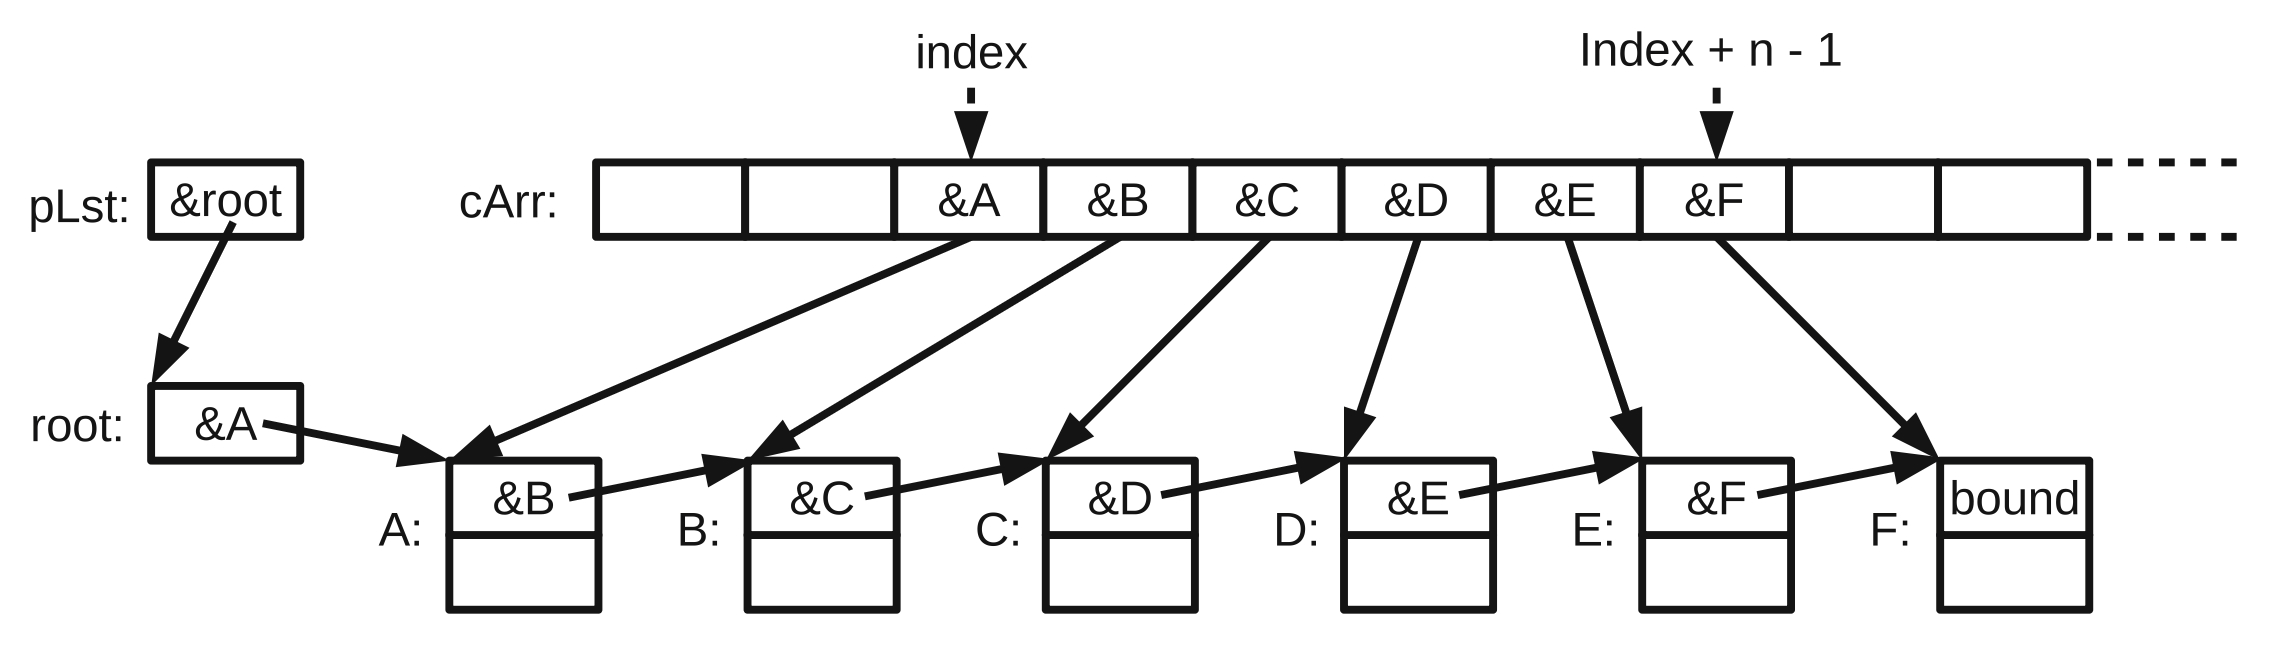
\includegraphics[width=\linewidth]{images/list-serialized}
    \caption{
        Vizualize serializace spojového seznamu. \\
        Převzato z článku Ghosts for Lists: A Critical Module of Contiki Verified in Frama\mbox{-}C~\cite{FCGhostsForLists}.
    }
    \label{fig:linked-list-serialization}
\end{figure}

Serializace stromu, ve speciálním případě binární haldy,
lze provést pomocí mapování prvků stromu do indexů pole dle následujícího vzorce.
Pokud je prvek na indexu $i$, pak levý potomek je na indexu $2i + 1$ a pravý potomek je na indexu $2i + 2$.
Rodičovský prvek je na indexu $\lfloor \frac{i - 1}{2} \rfloor$.
V binární haldě nemůže nastat situace s prázdným nepoužitým uzlem a pole se tedy vždy plní korektně
od nejnižšího indexu po nejvyšší.
Obecné stromy by s tímto principem nemohly být serializovány,
protože je možné, že některé uzly budou prázdné a nebudou mít žádného potomka.
Řešení, může být například nepoužívat jednoduchou serializaci prvků stromu do pole,
ale používat rozšířenou strukturu v serializovaném poli, která bude určovat,
zdali je daný prvek platný nebo ne.
Indexace prvků v poli by tímto přístupem byla zachována,
pouze důkazy používající tuto strukturu by musely při každém přístupu na prvek stromu
zkontrolovat, zdali je prvek platný nebo ne.
Na takto serializovaných stromech by bylo jednoduché provádět důkazy,
jelikož všechny prvky v poli jsou oddělené a tedy splňují podmínku oddělené paměti.
Predikáty popisující vlastnosti stromu by museli ale obsahovat kontrolu,
zdali je daný prvek v poli platný nebo ne.

% TODO: nebo ne -> a nebo ne?

Nevýhoda serializace obecných stormů do pole je ta, že řídké stromy budou zabírat
násobně více paměti, než je potřeba.
V nejhorším případě, kdy by pomocí této metody byl zakódován strom obsahující řetězec \texttt{n} pravých uzlů,
by serializované pole reprezentující tento strom mělo velikost $2^n~-~1$ s~$2^n~-~n$ neplatnými uzly.
Další nevýhoda serializace stromových struktu spočívá v složitosi
tvořených predikátů a vlastností stromu.
Serializací ztrácíme lokalitu problému a musíme lokálnost převést na práci s indexy v poli.


TODO: přidat více myšlenek o ztrátě lokálnosti

TODO: přídat příklad serializace binárního stromu do pole? (ne AVL)

% TODO: pridat nedelitelnou mezeru tak, aby nebyly jedno-znaky na konci radku samy

%why3 config detect
%Found prover Alt-Ergo version 2.5.3, OK.
%Found prover Alt-Ergo version 2.5.3 (alternative: BV)
%Found prover Alt-Ergo version 2.5.3 (alternative: counterexamples)
%Found prover CVC4 version 1.8 (alternative: strings+counterexamples)
%Found prover CVC4 version 1.8 (alternative: strings)
%Found prover CVC4 version 1.8 (alternative: counterexamples)
%Found prover CVC4 version 1.8, OK.
%7 prover(s) added
%Save config to /home/parallels/.why3.conf


%2.3.3 Model Selection
%These options modify the underlying memory model that is used for computing weakest
%preconditions. See chapter 3 for details. Models are identified by a combination of selectors
%which are defined below:
%Selector Description
%Hoare Select Hoare memory model.
%Typed Select Typed memory model with limited casts.
%cast Select Typed memory model with unlimited casts (unsound).
%nocast Select Typed memory model with no casts.
%raw Disable the combination of memory models.
%var Combination of memory models based on variable analysis.
%ref Activate the detection of pointer variables used for reference passing style.
%caveat Caveat memory model (see 3.7).
%int Use machine integers when overflows and downcasts might occurs.
%nat Integer model without bounds (no overflow assumed).
%float Use floating-point operations.
%real Use mathematical reals instead of floating point.

\chapter{Stainless}
\label{ch:stainless}

Stainless je nástroj pro ověřování korektnosti programů napsaných v jazyce Scala.
Scala je staticky typovaný jazyk, který je založen na jazyce Java.
Scala podporuje objektově orientované programování i funkcionální styl programování.
Nicméně podporovaný je hlavně funkcionální styl programování a některé konstrukce
imperativního programování jsou podporovány pomocí transformací, které jsou součástí
předzpracování zdrojového kódu~\cite{StainlessDocs}.

Stainless stejně jako Frama\mbox{-}C používá SMT řešiče pro dokazování vlastností programů.
Místo platformy Why3 ale používá vlastní mezivrstvu nazvanou Inox.
Inox podporuje generování důkazů pro externí SMT řešiče Z3, CVC4 a CVC5.
Interní řešič Princess, napsaný v jazyce Scala, je součástí distribuce a je ho tedy možné použít
i v případě, kdy není k dispozici žádný externí SMT řešič~\cite{InoxSolver}.

\section{Anotace}
\label{sec:stainless-annotations}

Stainless podporuje podobný styl anotování kódu jako Frama\mbox{-}C\@.
Není ale potřeba používát speciální komentáře pro anotace,
ale je možné použít přímo jazyk Scala.
Všechny anotace jsou umístěny jako spustitelný Scala kód a nebo jako dekorátory před funkcemi.

Anotace \texttt{require} zajišťuje, že daná podmínka musí být splněna před spuštěním funkce.
Příklad použití je zobrazen v ukázce~\ref{lst:stainless-require},
kde je deklarována funkce \texttt{my\_function} s dvěma celočíselnými parametry.
Podmínka spuštění této funkce je, že oba parametry musí být ostře větší než 0.

\begin{listing}[H]
  \begin{minted}{scala}
  def my_function(x: Int, y: Int): Int = {
    require(x > 0 && y > 0)
    ...
  }
  \end{minted}
  \caption{Příklad použití anotace \texttt{require}}
  \label{lst:stainless-require}
\end{listing}

Anotace \texttt{ensuring} zajišťuje, že po spuštění funkce budou splněné dané vlastnosti.
Ensuring přijímá jako argument funkci o jednom parametru,
která vrací hodnotu typu \texttt{Boolean}.
Parametrem této funkce je výstupní hodnota funkce,
která je na ukázce~\ref{lst:stainless-ensuring} pojmenována \texttt{res}.

\begin{listing}[H]
  \begin{minted}{scala}
  def my_function(x: Int, y: Int): Int = {
    ...
  }.ensuring(res => res > 0)
  \end{minted}
  \caption{Příklad použití anotace \texttt{ensuring}}
  \label{lst:stainless-ensuring}
\end{listing}

\subsection{Cykly}
\label{subsec:stainless-loops}

Cykly v jazyce Scala jsou jedním z imperativních prvků,
které Stainless musí transformovat na funkcionální styl.
Stejně jako při použití Frama\mbox{-}C je potřeba použít invarianty cyklu,
popisující vlastnosti cyklu.
Také je potřeba definovat variant cyklu,
pomocí kterého lze rozhodnout o konečnost cyklu.
Stainless posktytuje možnost definovat invariant pomocí klíčového slova \texttt{invariant}
umístěného za deklarací cyklu.
Variant je označen pomocí klíčového slova \texttt{decreases} na začátku těla cyklu.
Ukázka~\ref{lst:stainless-loop} zobrazuje jednoduchý příklad cyklu s použitím invariantu i variantu.
Při zápisu invariantu je nutné cyklus obalit do závorek,
jelikož Stainless používá pro integraci tohoto klíčového slova
implicitní konverzi z typu \texttt{Unit} na typ \texttt{InvariantFunction}~\cite{StainlessDocs}.

\begin{listing}[H]
  \begin{minted}{scala}
  def my_loop(x: Int): Int = {
    var i = x

    (while (i > 0) {
      decreases(i)

      i -= 1
    }).invariant(i >= 0)

    i
  }
  \end{minted}
  \caption{Příklad použití cyklu s invariantem a variantem}
  \label{lst:stainless-loop}
\end{listing}

\subsection{Pattern matching}
\label{subsec:stainless-pattern-matching}

Scala podporuje takzvaný pattern matching,
jehož funkce je podobná konstrukci \texttt{switch} v jazyce~C s několika vylepšeními.
Pomocí tohoto mechanismu je možné elegantně zpracovávat různé varianty datových typů.
Dokonce je možné rozpoznávat i složené datové typy pomocí destrukturizace.
Stainless také podporuje pattern matching a v následující kapitole s jeho pomocí
popíšeme implementaci AVL stromu~\cite{scalaPatternMatching}.

Scala podporuje koncept algebrických datových typů
a takzvaných \textit{case classes}.
Příkladem může být následující ukázka~\ref{lst:stainless-case-class},
kde je definována abstraktní třída \texttt{AVLTree} a dvě podtřídy \texttt{Node} a \texttt{Leaf},
které budou detailně popsány v kapitole~\ref{sec:stainless-avl}.
Přidáním příznaku \texttt{sealed} před definici třídy
je možné zajistit, že všechny podtřídy budou definované v rámci stejného souboru.

Kombinací pattern matchingu a \texttt{case class} je možné elegantně zpracovávat různé varianty datových typů.
Například pomocí kódu z ukázky~\ref{lst:stainless-pattern-matching-case-class}
je možné definovat funkci \texttt{content},
která pomocí pattern matchingu vypočítá množinu prvků obsažených v AVL stromu.

\begin{listing}[H]
  \begin{minted}{scala}
  sealed abstract class AVLTree {
    def content: Set[Int] = this match {
      case Leaf() => Set.empty
      case Node(v, l, r, _) => l.content ++ Set(v) ++ r.content
    }
  }
  \end{minted}
  \caption{Příklad použití pattern matchingu s \texttt{case class}}
  \label{lst:stainless-pattern-matching-case-class}
\end{listing}

Pattern matchingu bez Stainless může v některých případech vyvolat
varování o neúplnosti pattern matchingu, pokud \texttt{match} nezachycuje všechny \texttt{case class}
a neobsahuje fallback variantu pomocí konstrukce \texttt{case \_},
Toto varování Stainless vylepšuje a přidává kontext o spouštění funkce.
Pokud tedy v aktuálním kontextu některé případy nemohou nikdy nastat,
Stainless potlačí varování o neúplnosti pattern matchingu.

\section{Protipříklady}
\label{sec:stainless-counterexamples}

Velkou výhodou oproti Frama\mbox{-}C při vývoji důkazů pomocí Stainless je,
že Stainless v základní instalaci podporuje generování protipříkladů.
Protipříklad je konkrétní vstupní hodnota nebo nastavení proměnných,
které vedou k porušení kontraktu funkce.

Následující ukázka~\ref{lst:stainless-incorrect-intmax} zobrazuje
jednoduchou funkci \texttt{int\_max}, která vrací větší z dvou čísel.
Tato funkce je záměrně implementovana špatně,
aby bylo možné ukázat generování protipříkladů.
Definice kontraktu \texttt{ensuring} zajišťuje,
že výsledek volání funkce bude hodnota větší nebo rovna oběma vstupním parametrům.
Žádné vstupní podmínky (předpoklady) nejsou definované,
Stainless tedy předpokládá, že vstupní hodnoty jsou libovolné celočíselné hodnoty.
Pomocí příkazu~\ref{lst:stainless-incorrect-intmax-run}
lze spustit analýzu tohoto programu.

\begin{listing}[H]
  \begin{minted}{bash}
  def int_max(x: Int, y: Int): Int = {
    if (x > y) x else 0
  }.ensuring(res => res >= x && res >= y)
  \end{minted}
  \caption{Nesprávně implementovaná funkce \texttt{int\_max}}
  \label{lst:stainless-incorrect-intmax}
\end{listing}

\begin{listing}[H]
  \begin{minted}{console}
  stainless snippets/counterexample.scala
  \end{minted}
  \caption{Příkaz pro spuštění analýzy protipříkladů}
  \label{lst:stainless-incorrect-intmax-run}
\end{listing}

Výsledek analýzy z výpisu~\ref{lst:stainless-incorrect-intmax-result} ukazuje,
že pro vstupní hodnoty $x = -2147483648$ a $y = 2147483646$
je výstupní hodnota $0$, což je v rozporu s kontraktem funkce.
Stainless tyto protipříklady generuje automaticky,
ale již neprovádí jejich minimalizaci.

\begin{listing}[H]
  \begin{minted}{console}
  ...
  [Warning ] snippets/counterexample.scala:6:23:  => INVALID
               if (x > y) x else 0
                                 ^
  [Warning ] Found counter-example:
  [Warning ]   x: Int -> -2147483648
  [Warning ]   y: Int -> 2147483646
  ...
  \end{minted}
  \caption{Výstup analýzy s protipříkladem pro funkci \texttt{int\_max}}
  \label{lst:stainless-incorrect-intmax-result}
\end{listing}

Velmi užitečná je podpora protipříkladů i pro složitější datové struktury
jako například algebrické datové typy.
Například pro AVL strom, který bude popsán později v této kapitole,
byl v průběhu tvorby důkazu vygenerován protipříklad podobný jako z výpisu~\ref{lst:stainless-avl-counterexample},
ve kterém Stainless přesně popisuje protipříklad s kombinací datových typů \texttt{Node} a \texttt{Leaf}.
Zároveň je správně dodržena podmínka na výšku uzlu, která musí být ostře větší než 0.

\begin{listing}[H]
  \begin{minted}{console}
  [Warning ] Found counter-example:
  [Warning ]   thiss: AVLTree -> Node(0, Leaf(), Leaf(), 1)
  \end{minted}
  \caption{Výstup analýzy s protipříkladem pro AVL strom}
  \label{lst:stainless-avl-counterexample}
\end{listing}

% https://epfl-lara.github.io/stainless/genc.html
% The support for classes is restricted to non-recursive ones so that instances of such data-types live on the stack.
% ---
% Currently the memory model is limited to stack allocation and global state.
% Hence, no dynamic allocation is done using malloc function family.

% --genc does not support recursive data types = src/stainless/LinkedList.scala:41:12: Cons and other recursive types are not supported

\section{Ověřená implementace AVL stromu}
\label{sec:stainless-avl}

Datová struktura AVL stromu je rozšířením binárního vyhledávacího stromu,
který ale zajišťuje, že rozdíl výšek levého a pravého podstromu je maximálně 1.
Jedná se tedy o relaxovanou podmínku pro vyváženost stromu.
Tato datová struktura je velmi efektivní pro vyhledávání, vkládání a mazání prvků,
které mají pouze logaritickou složitost~\cite{Pruvodce22}.

Následující výpis~\ref{lst:stainless-avl-interface} zobrazuje rozhraní AVL stromu,
které je implementováno v jazyce Scala a následně ověřeno pomocí Stainless.
Datová struktura obsahuje základní operace pro vkládání, mazání a hledání prvku.
Jednotlivé funkce jsou korektně implementované a pomocí Stainless je možné ověřit jejich korektnost.
Třída \texttt{AVLTree} je abstraktní třída, která definuje základní vlastnosti AVL stromu
a podtřídy \texttt{Node} a \texttt{Leaf} implementují konkrétní chování stromu.
Zároveň je v kódu často používán pattern matching,
který umožňuje elegantně zpracovávat různé varianty situací, které mohou nastat.
List (Leaf) je prázdný uzel, který nemá žádné hodnoty a má výšku 0.
Jedná se o prázdný prvek, podobně jako by v jazyce C byl použit ukazatel \texttt{NULL}.
Nejedná se tedy o poslední platný uzel stromu, ale o zvláštní prvek, který nemá žádnou hodnotu.

\begin{listing}[H]
    \begin{minted}{scala}
    import stainless.lang._
    import stainless.collection._
    import stainless.annotation._

    def int_max(x: Int, y: Int): Int = ...

    sealed abstract class AVLTree {
      def content: Set[Int] = ...
      def height: Int = ...
      def balanceFactor: Int = ...
      def hasBinarySearchTreeStructure: Boolean = ...
      def hasAVLTreeStructure: Boolean = ...
      def isBalanced: Boolean = ...
      def isAVLTree: Boolean = ...
      def contains(x: Int): Boolean = ...
      def insert(x: Int): AVLTree = ...
      def delete(x: Int): AVLTree = ...
    }

    case class Leaf() extends AVLTree

    case class Node
    (
      value: Int,
      left: AVLTree,
      right: AVLTree,
      _height: Int
    ) extends AVLTree {
      require(_height > 0)

      def min: Int = ...
      def max: Int = ...
      def rotateLeft: Node = ...
      def rotateRight: Node = ...
      def rotateLeftRight: Node = ...
      def rotateRightLeft: Node = ...
      def balance: Node = ...
    }
    \end{minted}
    \caption{Rozhraní AVL stromu}
    \label{lst:stainless-avl-interface}
\end{listing}

Tato kapitola postupně popíše jednotlivé funkce a popíše důkazy jejich korektnosti.

Na začátku kódu je jednoduchá funkce \texttt{int\_max}, která vrací větší z dvou čísel.
Jedná se o pomocnou funkci na celých číslech, která se používá v dalších funkcích.
Stainless nepodporuje funkci \texttt{x max y} ze standardní knihovny,
proto je potřeba použít vlastní implementaci.

Ukázka~\ref{lst:stainless-avl-helper} zobrazuje pomocné funkce pro AVL strom.
První z nich je \texttt{content}, která vrací množinu prvků v AVL stromu.
Pomocí pattern matchingu se zjistí, zdali aktuálně zpracovávaný uzel je list nebo uzel.
Pokud je to list, vrátí se prázdná množina.
V případě uzlu se rekurzivně zavolá funkce \texttt{content} na levém a pravém podstromu
a spojí se dohromady do množiny s hodnotou uloženou v aktuálním uzlu.
Druhá funkce \texttt{height} vrací výšku stromu.
Listy stromu mají výšku 0 a uzly mají výšku uloženou v proměnné \texttt{\_height} (čtvrtý argument konstruktoru).
Třetí funkce \texttt{balanceFactor} vrací vyváženost stromu.
Listy jsou vždy vyvážené a uzly mají vyváženost počítanou jako rozdíl výšky pravého a levého podstromu.
V důkazech je použita tato vlastnost pro kontrolu vyváženosti stromu.

\begin{listing}[H]
  \begin{minted}{scala}
  def content: Set[Int] = this match {
    case Leaf() => Set.empty
    case Node(v, l, r, _) => l.content ++ Set(v) ++ r.content
  }

  def height: Int = this match {
    case Leaf() => 0
    case Node(_, _, _, h) => h
  }

  def balanceFactor: Int = {
    this match {
      case Leaf() => 0
      case Node(_, l, r, _) => r.height - l.height
    }
  }
  \end{minted}
  \caption{Pomocné funkce pro AVL strom}
  \label{lst:stainless-avl-helper}
\end{listing}

Jelikož je AVL strom nadstavbou binárního vyhledávacího stromu,
je potřeba zajistit, že splňuje všechny vlastnosti binárního vyhledávacího stromu.
K tomu slouží funkce \texttt{hasBinarySearchTreeStructure} zobrazená ve výpisu~\ref{lst:stainless-avl-bst},
která kontroluje hodnoty v uzlech a podmínky pro binární vyhledávací stromy.
Konkrétně, že levý podstrom obsahuje pouze hodnoty menší než hodnota aktuálního uzlu
a pravý podstrom pouze hodnoty větší než hodnota aktuálního uzlu.
Listy jsou automaticky označeny jako binární vyhledávací stromy (prázdný strom).
U uzlů se rekurzivně je nutné rekurzivně ověřit platnost pravidel pro
binární vyhledávací stromy na levém a pravém podstromu
a poté kontrolovat pravidlo pro binární vyhledávací stromy.

\begin{listing}[H]
  \begin{minted}{scala}
  def hasBinarySearchTreeStructure: Boolean = this match {
    case Leaf() => true
    case Node(v, l, r, _) => {
      l.hasBinarySearchTreeStructure &&
        r.hasBinarySearchTreeStructure &&
        // Ensure that the AVL
        //   has a binary search tree structure
        forall((x: Int) =>
          l.content.contains(x) ==> x < v
        ) &&
        forall((x: Int) =>
          r.content.contains(x) ==> x > v
        )
    }
  }
  \end{minted}
  \caption{Funkce pro kontrolu struktury binárního vyhledávacího stromu}
  \label{lst:stainless-avl-bst}
\end{listing}

Funkce \texttt{hasAVLTreeStructure} z výpisu~\ref{lst:stainless-avl-avl}
popisuje strukturu AVL stromu.
Tato funkce kontroluje, že prvky v AVL stromu jsou správně uspořádány.
Konkrétně je omezena hloubka stromu na maximálně \texttt{Int.MaxValue}
a výška stromu musí být správně vypočítaná (o jedna větší než maximální výška z podstromů).

\begin{listing}[H]
  \begin{minted}{scala}
  def hasAVLTreeStructure: Boolean = this match {
    case Leaf() => true
    case Node(v, l, r, _) => {
      l.hasAVLTreeStructure &&
        r.hasAVLTreeStructure &&
        // Ensure that the height of the tree
        //  is at most (at root) is Int.MaxValue
        l.height < Int.MaxValue &&
        r.height < Int.MaxValue &&
        // Ensure that the height of the tree is correct
        height == 1 + (l.height < r.height match {
          case true => r.height
          case false => l.height
        })
    }
  }
  \end{minted}
  \caption{Funkce pro kontrolu struktury AVL stromu}
  \label{lst:stainless-avl-avl}
\end{listing}

Funkce \texttt{isBalanced} z výpisu~\ref{lst:stainless-avl-balanced}
ověřuje, zdali je AVL strom vyvážený.
Kontroluje, zdali je rozdíl výšek pravého a levého podstromu
v rozsahu $[-1, 1]$.
Tato vývaženost musí rekurzivně platit pro všechny uzly v AVL stromu.

\begin{listing}[H]
  \begin{minted}{scala}
  def isBalanced: Boolean = this match {
    case Leaf() => true
    case Node(v, l, r, _) => {
      l.isBalanced &&
        r.isBalanced &&
        // Ensure that the balance factor
        //   is within [-1, 1]
        balanceFactor >= -1 &&
        balanceFactor <= 1
    }
  }
  \end{minted}
  \caption{Funkce pro ověření vyváženosti AVL stromu}
  \label{lst:stainless-avl-balanced}
\end{listing}

Funkce \texttt{isAVLTree} z výpisu~\ref{lst:stainless-avl-isavl}
ověřuje, že AVL strom splňuje všechny výše uvedené vlastnosti dohromady.

\begin{listing}[H]
  \begin{minted}{scala}
  def isAVLTree: Boolean = this match {
    case Leaf() => true
    case Node(v, l, r, h) => {
      l.isAVLTree &&
        r.isAVLTree &&
        hasBinarySearchTreeStructure &&
        hasAVLTreeStructure &&
        isBalanced
    }
  }
  \end{minted}
  \caption{Funkce pro ověření struktury AVL stromu}
  \label{lst:stainless-avl-isavl}
\end{listing}

Funkce \texttt{contains} z výpisu~\ref{lst:stainless-avl-contains}
ověřuje, zdali je daný prvek součástí AVL stromu.
Předpokladem spuštění této funkce je, že je spuštěna pouze na platném AVL stromu.
Následek popisující výsledek funkce zajišťuje,
že výsledek spuštění této funkce je stejný jako kontrola obsahu stromu pomocí množinové operace (\texttt{content.contains(x)}).

\begin{listing}[H]
  \begin{minted}{scala}
  def contains(x: Int): Boolean = {
    require(isAVLTree)
    this match {
      case Leaf() => false
      case Node(v, l, r, _) => {
        if (x == v) true
        else if (x < v) l.contains(x)
        else r.contains(x)
      }
    }
  }.ensuring(res => res == content.contains(x))
  \end{minted}
  \caption{Funkce pro kontrolu přítomnosti prvku v AVL stromu}
  \label{lst:stainless-avl-contains}
\end{listing}

Funkce \texttt{insert} z výpisu~\ref{lst:stainless-avl-insert}
provádí vložení prvku do AVL stromu.
V případě prázdného stromu se vytvoří nový uzel s danou hodnotou a výškou 1.
Pokud je strom již naplněn,
je potřeba zjistit, zdali prvek již ve stromu není.
Pokud není, je potřeba ho vložit na správné místo a případně provést opravu vyváženosti pomocí rotací.
Funkce \texttt{balance} bude představena později.
Prozatím stačí říci, že se jedná o funkci,
která dokáže opravit AVL strom i v případě,
kdy je balanční faktor aktuálního vrcholu v rozsahu $[-2, 2]$.

\begin{listing}[H]
  \begin{minted}{scala}
  def insert(x: Int): AVLTree = {
    require(isAVLTree)
    require(height < Int.MaxValue)

    this match {
      case Leaf() => Node(x, Leaf(), Leaf(), 1)
      case Node(v, l, r, _) => {
        if (x == v) this
        else if (x < v) {
          val newLeft = l.insert(x)
          Node(
            v, newLeft, r,
            1 + int_max(newLeft.height, r.height)
          ).balance
        } else {
          val newRight = r.insert(x)
          Node(
            v, l, newRight,
            1 + int_max(l.height, newRight.height)
          ).balance
        }
      }
    }
  }.ensuring(res =>
    res.isAVLTree &&
      (res.height == height || res.height == height + 1) &&
      res.content == content ++ Set(x)
  )
  \end{minted}
  \caption{Funkce pro vložení prvku do AVL stromu}
  \label{lst:stainless-avl-insert}
\end{listing}

Funkce \texttt{delete} z výpisu~\ref{lst:stainless-avl-delete}
provádí odstranění prvku z AVL stromu.
Jedná se o nejkomplexnejší z představených funkcí.
Pokud je aktuálně zpracovávaný uzel hledaný prvek na odstranění (\texttt{x == v}),
je potřeba rozlišit čtyři případy dle podstromů daného uzlu.
Pokud jsou oba podstromy prázdné, vrátí se instance listu (prázdný strom).
Vrácení prázdného listu je vlastně nahrazení daného vrcholu prázdným stromem.
Pokud pravý nebo levý podstrom zaplněný (ale ne oba),
vrátí se ten podstrom, který není prázdný.
Pokud jsou oba podstromy zaplněné,
je potřeba najít minimální prvek v pravém podstromu (následník),
odstranit ho z pravého podstromu
a vytvořit nový uzel s hodnotou následníka, stejným levým podstromem
a novým pravým podstromem, kde byl následník odstraněn.
V případech kdy je hledaný prvek menší nebo větší než hodnota aktuálního uzlu
je potřeba rekurzivně zavolat funkci \texttt{delete} na levém nebo pravém podstromu
a po provedení odstranění nebo ukončení v případě, kdy prvek není ve stromu,
je potřeba vytvořit nový uzel s novým levým nebo pravým podstromem
a provést opravu vyváženosti pomocí funkce \texttt{balance}.
Následky této funkce zajišťují, že se vždy vrátí korektní AVL strom
a že výška stromu se buď nezmění nebo se sníží maximálně o 1.
Zároveň je zajištěno, že obsah stromu je stejný jako v původním stromu,
s výjimkou odstraněného prvku.

\begin{listing}[H]
  \begin{minted}{scala}
  def delete(x: Int): AVLTree = {
    require(isAVLTree)
    this match {
      case Leaf() => this
      case Node(v, l, r, _) => {
        if (x == v) {
          (l, r) match {
            case (Leaf(), Leaf()) => Leaf()
            case (Leaf(), Node(_, _, _, _)) => r
            case (Node(_, _, _, _), Leaf()) => l
            case (Node(_, _, _, _), rn: Node) => {
              val m = rn.min
              val newRight = r.delete(m)
              Node(
                m, l, newRight,
                1 + int_max(l.height, newRight.height)
              ).balance
            }
          }
        } else if (x < v) {
          val newLeft = l.delete(x)
          Node(
            v, newLeft, r,
            1 + int_max(newLeft.height, r.height)
          ).balance
        } else {
          val newRight = r.delete(x)
          Node(
            v, l, newRight,
            1 + int_max(l.height, newRight.height)
          ).balance
        }
      }
    }
  }.ensuring(res =>
    res.isAVLTree &&
      (res.height == height || res.height == height - 1) &&
      res.content == content -- Set(x)
  )
  \end{minted}
  \caption{Funkce pro odstranění prvku z AVL stromu}
  \label{lst:stainless-avl-delete}
\end{listing}

Předchozí funkce \texttt{delete} využívala funkci \texttt{min} z výpisu~\ref{lst:stainless-avl-min-max},
která vrací minimální prvek v AVL stromu.
Pro kompletnost je na uzlech definována i funkce \texttt{max},
která vrací maximální prvek v AVL stromu.

\begin{listing}[H]
  \begin{minted}{scala}
  def min: Int = {
    require(isAVLTree)
    this match {
      case Node(v, Leaf(), _, _) => v
      case Node(_, l: Node, _, _) => l.min
    }
  }.ensuring(res =>
    content.contains(res) &&
      forall((x: Int) =>
        (content.contains(x) && x != res) ==> x > res
      )
  )

  def max: Int = {
    require(isAVLTree)
    this match {
      case Node(v, _, Leaf(), _) => v
      case Node(_, _, r: Node, _) => r.max
    }
  }.ensuring(res =>
    contains(res) &&
      forall((x: Int) =>
        (contains(x) && x != res) ==> x < res
      )
  )
  \end{minted}
  \caption{Funkce pro zjištění minimálního a maximálního prvku v AVL stromu}
  \label{lst:stainless-avl-min-max}
\end{listing}

Funkce \texttt{rotateLeft} a \texttt{rotateRight}
z výpisu~\ref{lst:stainless-avl-rotate}
provádějí základní rotace uzlů v AVL stromu.
Tyto funkce jsou volány v případě, kdy je potřeba opravit vyváženost stromu
a zajišťují, že strom zůstane AVL stromem a jeho obsah se nezmění.
Vstupní podmínka těchto funkcí nemůže být pouze \texttt{isAVLTree},
jelikož \texttt{isAVLTree} zajišťuje, že strom je vyvážený,
což na místech v programu, kde se tyto funkce volají není zaručeno.
Následky spuštění těchto funkcí zaručují,
že strom bude správně vyvážen a obsah zůstane nezměněn.

\begin{listing}[H]
  \begin{minted}{scala}
  def rotateLeft: Node = {
    require(hasBinarySearchTreeStructure)
    require(hasAVLTreeStructure)
    require(left.isAVLTree && right.isAVLTree)
    require(balanceFactor == 2 && right.balanceFactor >= 0)

    right match {
      case Node(v, rl, rr, _) =>
        Node(
          v,
          Node(
            value, left, rl,
            1 + int_max(left.height, rl.height)
          ),
          rr,
          1 + int_max(
            1 + int_max(left.height, rl.height),
            rr.height
          )
        )
    }
  }.ensuring(res => res.content == content && res.isAVLTree)

  def rotateRight: Node = {
    require(hasBinarySearchTreeStructure)
    require(hasAVLTreeStructure)
    require(left.isAVLTree && right.isAVLTree)
    require(balanceFactor == -2 && left.balanceFactor <= 0)

    left match {
      case Node(v, ll, lr, _) =>
        Node(
          v,
          ll,
          Node(
            value, lr, right,
            1 + int_max(lr.height, right.height)
          ),
          1 + int_max(
            1 + int_max(lr.height, right.height),
            ll.height
          )
        )
    }
  }.ensuring(res => res.content == content && res.isAVLTree)
  \end{minted}
  \caption{Funkce pro jednoduché rotace uzlů v AVL stromu}
  \label{lst:stainless-avl-rotate}
\end{listing}

Dvojité rotace \texttt{rotateLeftRight} a \texttt{rotateRightLeft}
z výpisu~\ref{lst:stainless-avl-rotateLeftRight} a~\ref{lst:stainless-avl-rotateRightLeft}
reprezentují levo-pravou a pravo-levou rotaci uzlů v AVL stromu.

\begin{listing}[H]
  \begin{minted}{scala}
  def rotateLeftRight: Node = {
    require(hasBinarySearchTreeStructure)
    require(hasAVLTreeStructure)
    require(left.isAVLTree && right.isAVLTree)
    require(balanceFactor == -2 && left.balanceFactor == 1)

    left match {
      case Node(v, ll, lr, _) =>
        lr match {
          case Node(vlr, lrl, lrr, _) =>
            Node(
              vlr,
              Node(
                v, ll, lrl,
                1 + int_max(ll.height, lrl.height)
              ),
              Node(
                value, lrr, right,
                1 + int_max(lrr.height, right.height)
              ),
              1 + int_max(
                1 + int_max(ll.height, lrl.height),
                1 + int_max(lrr.height, right.height)
              )
            )
        }
    }
  }.ensuring(res => res.content == content && res.isAVLTree)
  \end{minted}
  \caption{Funkce pro levou-pravou rotaci uzlů v AVL stromu}
  \label{lst:stainless-avl-rotateLeftRight}
\end{listing}

\begin{listing}[H]
  \begin{minted}{scala}
  def rotateRightLeft: Node = {
    require(hasBinarySearchTreeStructure)
    require(hasAVLTreeStructure)
    require(left.isAVLTree && right.isAVLTree)
    require(balanceFactor == 2 && right.balanceFactor == -1)

    right match {
      case Node(v, rl, rr, _) =>
        rl match {
          case Node(vrl, rll, rlr, _) =>
            Node(
              vrl,
              Node(
                value, left, rll,
                1 + int_max(left.height, rll.height)
              ),
              Node(
                v, rlr, rr,
                1 + int_max(rlr.height, rr.height)
              ),
              1 + int_max(
                1 + int_max(left.height, rll.height),
                1 + int_max(rlr.height, rr.height)
              )
            )
        }
    }
  }.ensuring(res => res.content == content && res.isAVLTree)
  \end{minted}
  \caption{Funkce pro pravo-levou rotaci uzlů v AVL stromu}
  \label{lst:stainless-avl-rotateRightLeft}
\end{listing}

Poslední funkce \texttt{balance} z výpisu~\ref{lst:stainless-avl-balance}
provádí obecně opravu vyváženosti uzlu.
Rotace uzlů představené v předchozích výpisech
jsou striktně povolené pouze ve specifických případech rozdělených podle
balančního faktoru uzlu.
Obecná funkce \texttt{balance} přijímá k opravě jakýkoli uzel s balančním faktorem
v intervalu [-2, 2], kde pravý i levý strom jsou ale správně vyvážené AVL stromy.

Tento postup byl zvolen z důvodu usnadnění implementace předchozích funkcí \texttt{insert} a \texttt{delete}.
Volání jedné funkce ve včech scénářích, kde je potřeba vyvážit uzel stromu,
je implementačně i důkazově jednodušší než tuto logiku přenášet do zmíněných funkcí,
ve kterých by bylo nutné provést tuto logiku duplicitně.
Tento postup také umožňuje rychlejší dokončení důkazu korektnosti celého programu.

Funkce \texttt{balance} je úmysleně napsaná tak, aby opravila
jakýkoli uzel s nevývážeností v intervalu $[-2, 2]$ nehledě na to,
jak jsou vyvážené jeho podstromy.
Například operace \texttt{insert} nikdy nevygeneruje stav,
ve kterém by rodičovský uzel měl balanční faktor $2$ nebo $-2$
a zároveň potomek, ve kterém proběhlo přidání, tohoto uzlu měl balanční faktor $0$~\cite{Pruvodce22}.
Nicméně pro důkazní popis je tato situace,
kdy něco nemůže nastat, komplikovaně popsatelná.
Proto byla zvolena implementace této funkce tak,
aby se při zavolání \texttt{balance} na uzlu s balančním faktorem $2$ a balančním faktorem pravého syna $0$
zvolila levá rotace.
Výsledek rotace bude totiž AVL strom a jeho obsah zůstane stejný.
Případ balančního faktoru $-2$ a levém synovi s balančním faktorem $0$ je podobný,
pouze s pravou rotací.

\begin{listing}[H]
  \begin{minted}{scala}
  def balance: Node = {
    require(hasBinarySearchTreeStructure)
    require(hasAVLTreeStructure)
    require(left.isAVLTree && right.isAVLTree)
    require(-2 <= balanceFactor && balanceFactor <= 2)

    if (balanceFactor == 2) {
      if (right.balanceFactor == -1) rotateRightLeft
      else rotateLeft
    } else if (balanceFactor == -2) {
      if (left.balanceFactor == 1) rotateLeftRight
      else rotateRight
    } else this
  }.ensuring(res => res.content == content && res.isAVLTree)
  \end{minted}
  \caption{Funkce pro opravu vyváženosti uzlů v AVL stromu}
  \label{lst:stainless-avl-balance}
\end{listing}


\chapter*{Závěr}
\addcontentsline{toc}{chapter}{Závěr}
\markboth{Závěr}{Závěr}

Tato práce se zaměřila na důkladný popis nástrojů pro formální verifikaci programů,
které se zaměřují na různé programovací jazyky a programovací paradigmata.
Byl popsán základní princip fungování SMT řešičů společně se standardizovaným jazykem SMT-LIB\@.
Poté byl představen teoretický základ ve formě Hoareovy logiky a metody nejslabšího předpokladu,
které jsou základem pro deduktivní verifikaci programů.

Jedním z cílů bylo představit metody pro verifikaci dynamických rekurzivních datových struktur,
reprezentované na příkladu AVL stromu.
Pro vysvětlení problematiky důkazů těchto datových struktur
bylo prostředí Frama\mbox{-}C prozkoumáno do větší hloubky,
včetně architektury paměťových modelů a způsobu reprezentace oddělené paměti.
Bylo možné představit problematické oblasti,
které v současnosti zamezují jednoduchému popisu těchto datových struktur.
Zároveň byla popsána metoda kombinující axiomatický přístup a princip oddělené paměti,
které dohromady při správném použití umožňují verifikaci těchto struktur
bez zavedení velkých a složitých axiomů.
Tato kombinovaná metoda také umožňila začlenění a používání alokačních funkcí (například \texttt{malloc}),
což je velmi málo popisovaný problém v literatuře zabývající se Frama\mbox{-}C\@.

Stainless a jeho přístup k verifikaci dynamických datových struktur
byl bezproblémový a umožnil vcelku jednoduchou verifikaci AVL stromu.
Použité principy v důkazu této datové struktury jsou převoditelné
i na jiné datové struktury.

Závěřem je také vhodné zmínit, že dostupná literatura popisující prostředí Frama\mbox{-}C
je v současnosti bohatší než literatura popisující Stainless.
I přesto byla práce se Stainless příjemná a dokumentace dostačující.


\appendix\appendixinit % do not remove these two commands

%\chapter{Nějaká příloha}
%
%
%Sem přijde to, co nepatří do hlavní části.
 % include `appendix.tex' from `text/' subdirectory

\backmatter % do not remove this command

\printbibliography % print out the BibLaTeX-generated bibliography list

\chapter{Obsah příloh}
% Contents of the attachment

	\dirtree{%
		.1 /.
		.2 frama-c.
		.3 snippets/\DTcomment{ukázkové úryvky kódu pro Frama\mbox{-}C}.
		.2 stainless.
		.3 snippets/\DTcomment{ukázkové úryvky kódu pro Stainless}.
		.3 LinkedList.scala\DTcomment{ověřená struktura spojového seznamu}.
		.3 BinarySearchTree.scala\DTcomment{ověřená struktura binárního vyhledávacího stromu}.
		.3 AVLTree.scala\DTcomment{ověřená struktura AVL stromu}.
	}
 % include `medium.tex' from `text/' subdirectory

\end{document}
